%% ============================================================
%%  M.Tech Dissertation Phase-I progress report
%%  Kaustubh Pandey (2025PA17326), NSUT New Delhi
%%
%%  COMPILE WITH XeLaTeX.
%%  On Overleaf: Menu -> Compiler -> XeLaTeX.
%%
%%  Body font is TeX Gyre Termes, which has the same metrics as
%%  Times New Roman. If you compile locally on a machine that has
%%  the real Times New Roman installed, swap the \setmainfont line
%%  marked below.
%% ============================================================
\documentclass[12pt,a4paper]{article}

\usepackage{fontspec}
\usepackage{geometry}
\usepackage{setspace}
\usepackage{graphicx}
\usepackage{booktabs}
\usepackage{array}
\usepackage{amsmath}
\usepackage{enumitem}
\usepackage{fancyvrb}
\usepackage{titlesec}
\usepackage[labelformat=empty,font=normalsize,skip=6pt]{caption}
\usepackage{tocloft}
\usepackage[hidelinks]{hyperref}

%% ---- margins fixed by the department notice
\geometry{a4paper, left=1.5in, right=1.0in, top=1.0in, bottom=1.0in}

%% ---- fonts
\setmainfont{texgyretermes}[
  Extension      = .otf,
  UprightFont    = *-regular,
  BoldFont       = *-bold,
  ItalicFont     = *-italic,
  BoldItalicFont = *-bolditalic ]
%% If the line above ever fails, either of these also works:
%%   \setmainfont{TeX Gyre Termes}      % by font name
%%   \setmainfont{Times New Roman}      % local machine with the real font

%% Devanagari and IPA are shipped with the project so this builds anywhere.
\newfontfamily\devfont{NotoSansDevanagari-Regular.ttf}[Path=fonts/, Script=Devanagari]
\newfontfamily\ipafont{NotoSerif-Regular.ttf}[Path=fonts/]
\DeclareRobustCommand{\dev}[1]{{\devfont #1}}
\DeclareRobustCommand{\ipa}[1]{{\ipafont #1}}

%% ---- 1.5 line spacing throughout
\setstretch{1.5}
\setlength{\parskip}{4pt}
\setlength{\parindent}{0pt}

%% ---- heading sizes fixed by the notice
\titleformat{\section}{\normalfont\fontsize{14}{17}\bfseries}{}{0pt}{}
\titleformat{\subsection}{\normalfont\fontsize{12}{15}\bfseries}{}{0pt}{}
\titleformat{\subsubsection}{\normalfont\fontsize{12}{15}\bfseries\itshape}{}{0pt}{}
\titlespacing*{\section}{0pt}{14pt}{6pt}
\titlespacing*{\subsection}{0pt}{11pt}{4pt}
\titlespacing*{\subsubsection}{0pt}{9pt}{3pt}

%% ---- index pages
\renewcommand{\cftsecfont}{\bfseries}
\renewcommand{\cftsecpagefont}{\bfseries}
\setlength{\cftbeforesecskip}{3pt}
\setlength{\cftbeforesubsecskip}{1pt}
\renewcommand{\cftsecleader}{\cftdotfill{\cftdotsep}}
\setlength{\cftfigindent}{0pt}
\setlength{\cfttabindent}{0pt}

\setlength{\tabcolsep}{5pt}
\renewcommand{\arraystretch}{1.12}
\setlength{\emergencystretch}{2em}

\begin{document}
\thispagestyle{empty}
\begin{center}
\vspace*{0.2in}
{\fontsize{16}{20}\selectfont\bfseries Empirical Benchmarking of Neural Text-to-Speech Architectures for Indic Languages: Does Explicit Devanagari Grapheme-to-Phoneme Conversion Still Matter?}\\[0.5in]
This progress report is submitted in partial fulfilment of the requirements for the degree of\\[0.22in]
{\fontsize{14}{17}\selectfont\bfseries MASTER OF TECHNOLOGY}\\[0.06in]
in\\[0.06in]
Computer Science and Engineering – Artificial Intelligence\\[0.3in]
By\\[0.1in]
{\fontsize{13}{16}\selectfont\bfseries Kaustubh Pandey\quad(2025PA17326)}\\[0.3in]
Under the supervision of\\[0.1in]
\textbf{Dr. Shobha Bhatt}\\
\textbf{(Assistant Professor)}\\[0.28in]

\includegraphics[width=1.5in]{figures/nsut_logo.png}\\[0.28in]
Department of Computer Science and Engineering\\
Netaji Subhas University of Technology (NSUT)\\
New Delhi, India – 110078\\[0.12in]
\textbf{SEPTEMBER 2026}
\end{center}
\clearpage

\pagenumbering{roman}\setcounter{page}{2}
\pagestyle{plain}

\section*{\centering DECLARATION}
\addcontentsline{toc}{section}{Declaration}

I, \textbf{Kaustubh Pandey}, Roll No. \textbf{2025PA17326}, a student of Master of Technology in Computer Science and Engineering – Artificial Intelligence at the Department of Computer Science and Engineering, Netaji Subhas University of Technology (NSUT), New Delhi, hereby declare that the work presented in this Dissertation Phase-I progress report, entitled “Empirical Benchmarking of Neural Text-to-Speech Architectures for Indic Languages: Does Explicit Devanagari Grapheme-to-Phoneme Conversion Still Matter?”, is my own work carried out under the supervision of Dr. Shobha Bhatt, Assistant Professor.

I further declare that the corpora used in this work are publicly available research datasets and are cited as such, that all software libraries and pretrained model checkpoints used are cited in the references, and that every figure and table in this report was produced from measurements made by me on those corpora unless its caption states otherwise.

To the best of my knowledge and belief, this report contains no material previously published or written by another person, nor material which to a substantial extent has been accepted for the award of any other degree or diploma at this or any other institution, except where due acknowledgement has been made in the text. Any contribution made to this work by others is explicitly acknowledged.

I understand that any violation of the above will be cause for disciplinary action by the institute and may evoke penal action from the sources which have not been properly cited.

\vspace{0.35in}

\noindent Place: New Delhi \hfill Kaustubh Pandey

\vspace{0.28in}

\noindent Date:\textbackslash{} \textbackslash{}rule\{1.2in\}\{0.4pt\} \hfill Roll No. 2025PA17326

\vspace{0.28in}

\clearpage

\section*{\centering CERTIFICATE}
\addcontentsline{toc}{section}{Certificate}

This is to certify that the Dissertation Phase-I progress report entitled “Empirical Benchmarking of Neural Text-to-Speech Architectures for Indic Languages: Does Explicit Devanagari Grapheme-to-Phoneme Conversion Still Matter?”, submitted by \textbf{Kaustubh Pandey} (Roll No. \textbf{2025PA17326}) to the Department of Computer Science and Engineering, Netaji Subhas University of Technology (NSUT), New Delhi, in partial fulfilment of the requirements for the award of the degree of Master of Technology in Computer Science and Engineering – Artificial Intelligence, is a record of bona fide work carried out by the candidate under my supervision and guidance.

The candidate has completed the preparatory phase of the work described herein, comprising corpus profiling and standardisation, construction and validation of a Devanagari grapheme-to-phoneme front end, verification of the objective evaluation metrics, and specification of the full experimental matrix. In my opinion, the work has reached the standard required for the Phase-I evaluation.

To the best of my knowledge, the contents of this report have not been submitted, in part or in full, to any other university or institute for the award of any degree or diploma.

\vspace{0.35in}

\noindent Dr. Shobha Bhatt \hfill Head of Department

\vspace{0.28in}

\noindent (Assistant Professor) \hfill Department of Computer Science and Engineering

\vspace{0.28in}

\noindent Date:\textbackslash{} \textbackslash{}rule\{1.2in\}\{0.4pt\} \hfill Date:\textbackslash{} \textbackslash{}rule\{1.2in\}\{0.4pt\}

\vspace{0.28in}

\clearpage

\renewcommand{\contentsname}{\normalfont\centering TABLE OF CONTENTS}
\begin{singlespace}
\tableofcontents
\end{singlespace}
\clearpage

\renewcommand{\listfigurename}{\normalfont\centering LIST OF FIGURES}
\begin{singlespace}
\listoffigures
\addcontentsline{toc}{section}{List of Figures}
\vspace{0.25in}
\renewcommand{\listtablename}{\normalfont\centering LIST OF TABLES}
\listoftables
\addcontentsline{toc}{section}{List of Tables}
\end{singlespace}
\clearpage

\section*{\centering LIST OF ABBREVIATIONS}
\addcontentsline{toc}{section}{List of Abbreviations}
\begin{singlespace}
\begin{description}[leftmargin=1.5in,style=sameline,itemsep=0pt,parsep=0pt,topsep=4pt]
  \item[ASR] Automatic Speech Recognition
  \item[CFM] Conditional Flow Matching
  \item[DCT] Discrete Cosine Transform
  \item[DTW] Dynamic Time Warping
  \item[EBU] European Broadcasting Union
  \item[F0] Fundamental Frequency
  \item[fp16] Half-precision (16-bit) Floating Point
  \item[G2P] Grapheme-to-Phoneme
  \item[GAN] Generative Adversarial Network
  \item[GMM-HMM] Gaussian Mixture Model – Hidden Markov Model
  \item[GPU] Graphics Processing Unit
  \item[IPA] International Phonetic Alphabet
  \item[ITU] International Telecommunication Union
  \item[LUFS] Loudness Units relative to Full Scale
  \item[MAS] Monotonic Alignment Search
  \item[MCD] Mel-Cepstral Distortion
  \item[MFA] Montreal Forced Aligner
  \item[MMS] Massively Multilingual Speech
  \item[MOS] Mean Opinion Score
  \item[MPD] Multi-Period Discriminator
  \item[MRF] Multi-Receptive Field fusion
  \item[MSD] Multi-Scale Discriminator
  \item[NFC] Unicode Normalization Form C
  \item[NISQA] Non-Intrusive Speech Quality Assessment
  \item[ODE] Ordinary Differential Equation
  \item[RMSE] Root Mean Square Error
  \item[RTF] Real-Time Factor
  \item[SHA-256] Secure Hash Algorithm, 256-bit
  \item[TTS] Text-to-Speech
  \item[UTMOS] UTokyo-SaruLab Mean Opinion Score predictor
  \item[VAE] Variational Autoencoder
  \item[V/UV] Voiced / Unvoiced
  \item[WER] Word Error Rate
  \item[YAML] YAML Ain't Markup Language
\end{description}
\end{singlespace}
\clearpage

\section*{\centering ABSTRACT}
\addcontentsline{toc}{section}{Abstract}
Devanagari is an abugida, so every written consonant carries an unwritten inherent vowel, the schwa. Hindi deletes many of these in speech and keeps others, and the spelling does not say which. The conventional response is an explicit grapheme-to-phoneme front end that applies a deletion rule before any text reaches an acoustic model. Modern neural text-to-speech is trained end to end and may learn the same distinction from audio, in which case that front end is unnecessary engineering. No published study measures which of these is true, because none holds architecture, data, training budget, vocoder and evaluation fixed while varying only the input representation.

This work builds that measurement. FastSpeech 2, VITS and Matcha-TTS, drawn from three generative families, are to be trained on phonemic and on graphemic input under a provably identical budget, across a nested data ladder from nine hours down to ten minutes, with Marathi as a same-script control in which medial schwa deletion does not apply. That control separates a property of the script from one of the phonology.

This report covers the preparatory phase, which is complete. Both corpora were profiled from full passes rather than samples, standardised to $-23$ LUFS, and matched on a speaker identity recovered acoustically because neither dataset records it. Splits are frozen by salted hashing and regenerate byte for byte. The four-stage front end covers 870,547 phone tokens with zero unknown symbols, and Marathi’s inventory is a measured strict subset of Hindi’s. Both objective metrics were verified against analytic answers rather than merely executed. Three defects were found, the worst of which would have corrupted 16.5 per cent of Hindi word tokens on the phonemic arm alone. Seventeen runs totalling 136 GPU-hours are specified and budget-matched by assertion.

\vspace{6pt}\noindent\textit{Keywords:} text-to-speech, grapheme-to-phoneme conversion, schwa deletion, Devanagari, Hindi, Marathi, FastSpeech~2, VITS, Matcha-TTS, low-resource speech synthesis.
\clearpage
\pagenumbering{arabic}\setcounter{page}{1}

\section*{CHAPTER 1  INTRODUCTION}
\addcontentsline{toc}{section}{Chapter 1  Introduction}
\subsection*{1.1  Background}
\addcontentsline{toc}{subsection}{1.1  Background}
In Hindi speech, vowels decide how a word is pronounced and often what it means, but Hindi spelling does not tell you where a vowel is pronounced and where one is skipped. A classic example of the same comes from the words \textit{namak} (salt) and \textit{namkeen} (savoury). Both begin with the same three consonants, \dev{न}, \dev{म} and \dev{क}, yet one is pronounced \ipa{/nəmək/} and the other \ipa{/nəmkiːn/}. Both are written in Devanagari with no vowel sign after the second consonant, but one keeps the vowel there and the other drops it, and the spelling does not help you tell the two apart.

This is schwa deletion. Devanagari is an abugida, so every consonant that is written carries a hidden vowel sound, the schwa \ipa{ə}, and Hindi deletes many of them. The standard fix for the problem still comes from the iterative right-to-left rule given in a 2004 paper by Narasimhan, Sproat and Kiraz [1], which deletes a schwa lying between two consonants that are themselves flanked by vowels. It works well, but not perfectly, and the errors generally occur at morpheme boundaries and in loanwords. Arora et al. [2] later recast the task as supervised sequence labelling and improved on it.

Speech synthesis has progressed rapidly in the neural powered world, and the architectures to emerge on top are: FastSpeech 2 [3], a non-autoregressive transformer that needs explicit durations; VITS [4], which maps text to waveform through a variational autoencoder trained adversarially and learns its own alignment; and Matcha-TTS [5], which uses conditional flow matching to reach a quality equivalent to diffusion level models in far fewer steps. In cases where a spectrogram is produced, HiFi-GAN [6] turns it into audio.

In the fast paced race towards building local supportive AI, the resources available for Indic TTS have also improved, from the IIT Madras consortium recordings [7] through AI4Bharat's baselines [8] and IndicVoices-R [9] to MMS [10], whose pretrained VITS checkpoints cover both the languages chosen for this work, making fine tuning a realistic starting point. Another fact of note for this work is that Marathi uses the same script as Hindi and shares most of its phoneme inventory [11, 12], but does not apply Hindi's medial schwa deletion rule.

Figure 1.1 shows where all of this sits. A text-to-speech system is three stages: a front end that turns text into the symbols the model is trained on, an acoustic model that turns those symbols into a mel spectrogram, and a vocoder that turns the spectrogram into a waveform. The front end is the only stage this study varies.

\begin{figure}[htbp]
  \centering
  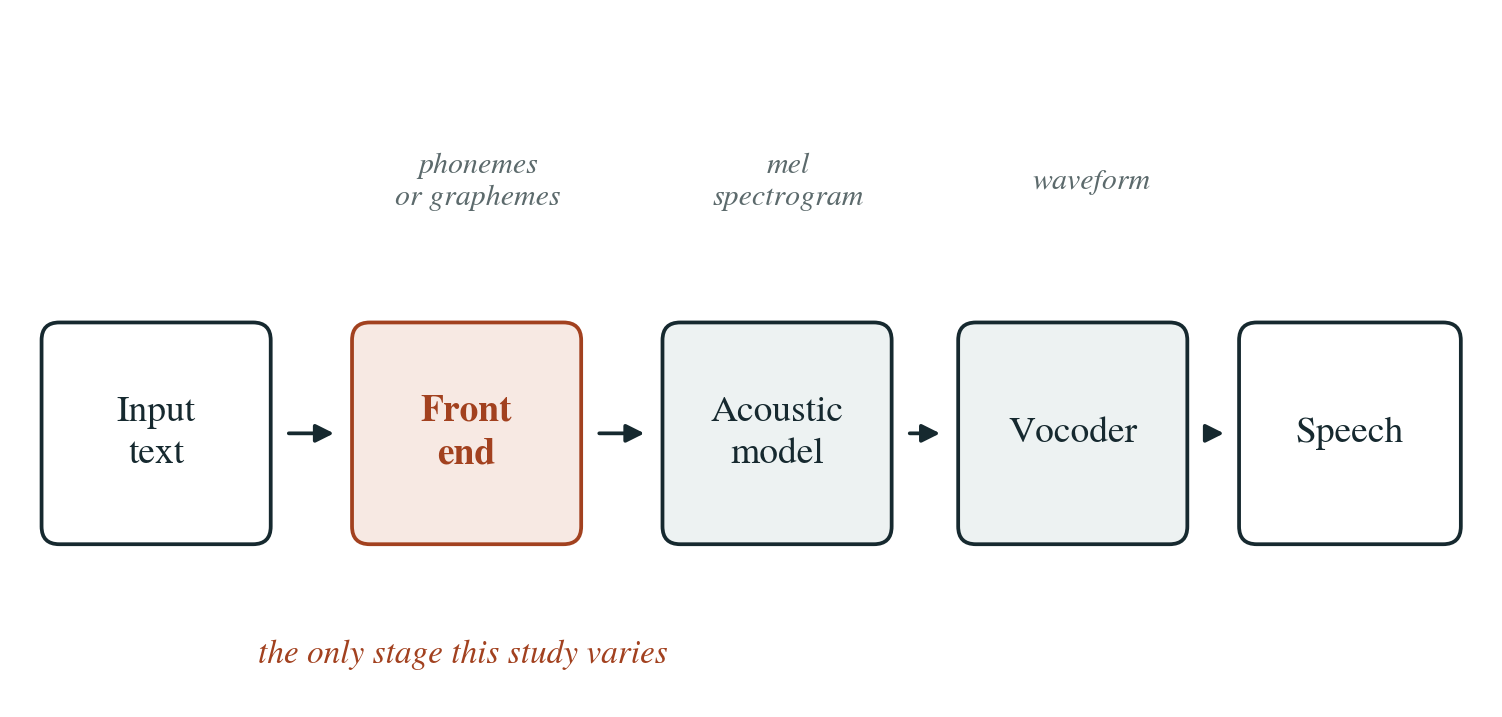
\includegraphics[width=3.85in]{figures/fig_1_2_tts_pipeline.png}
  \caption*{\textbf{Figure 1.1:}  The three stages of a neural text-to-speech system. With a phonemic front end the model is trained on phonemes, in which the schwa deletion has already happened. With a graphemic front end it is trained on Devanagari characters and has to learn the deletion from audio, if it learns it at all.}
  \addcontentsline{lof}{figure}{Figure 1.1: The three stages of a neural text-to-speech system}
\end{figure}

\subsection*{1.2  The Schwa Deletion Problem}
\addcontentsline{toc}{subsection}{1.2  The Schwa Deletion Problem}
Writing systems divide roughly three ways. An alphabet writes consonants and vowels as equal citizens, which is what the Latin script does. A syllabary gives each syllable a sign of its own, as Japanese kana does. An abugida writes consonants as full letters and writes vowels as marks attached to them, and it gives every consonant one default vowel that is never written at all [13]. Devanagari is an abugida and its default vowel is the schwa.

So \dev{क} is not the sound k. It is \ipa{/kə/}. To write a bare k you add a virama, giving \dev{क्}. To write some other vowel you add a matra, so \dev{का} is \ipa{/kaː/} and \dev{कि} is /ki/. Four further marks matter for a front end: the anusvara \dev{ं}, a nasal that takes the place of articulation of whatever follows it; the chandrabindu \dev{ँ}, which nasalises the vowel itself; the visarga \dev{ः}, realised as a voiceless breath; and the nukta \dev{़}, which marks a borrowed consonant. The anusvara is the first sign that a front end cannot be a lookup table, because resolving it means looking at the next segment.

The deletion rule itself is stated as V C \_ C V, applied iteratively from right to left [1]. In words, a schwa disappears when it sits between two consonants that each have a vowel on their far side. A separate and simpler rule deletes the word-final schwa, which in Hindi goes almost unconditionally. Two properties of the rule matter more than the rule itself. It is iterative, so deleting one schwa changes the context of its neighbour and can either enable or block the next deletion. And it runs right to left, because the word-final deletion has to happen first for the rest to come out correctly.

Figure 1.2 works both of our example words through the rule, step by step. The point of the pair is that the first three letters are identical and the pronunciation of the second one is not. Nothing in \dev{नमक} on its own tells you that.

\begin{figure}[htbp]
  \centering
  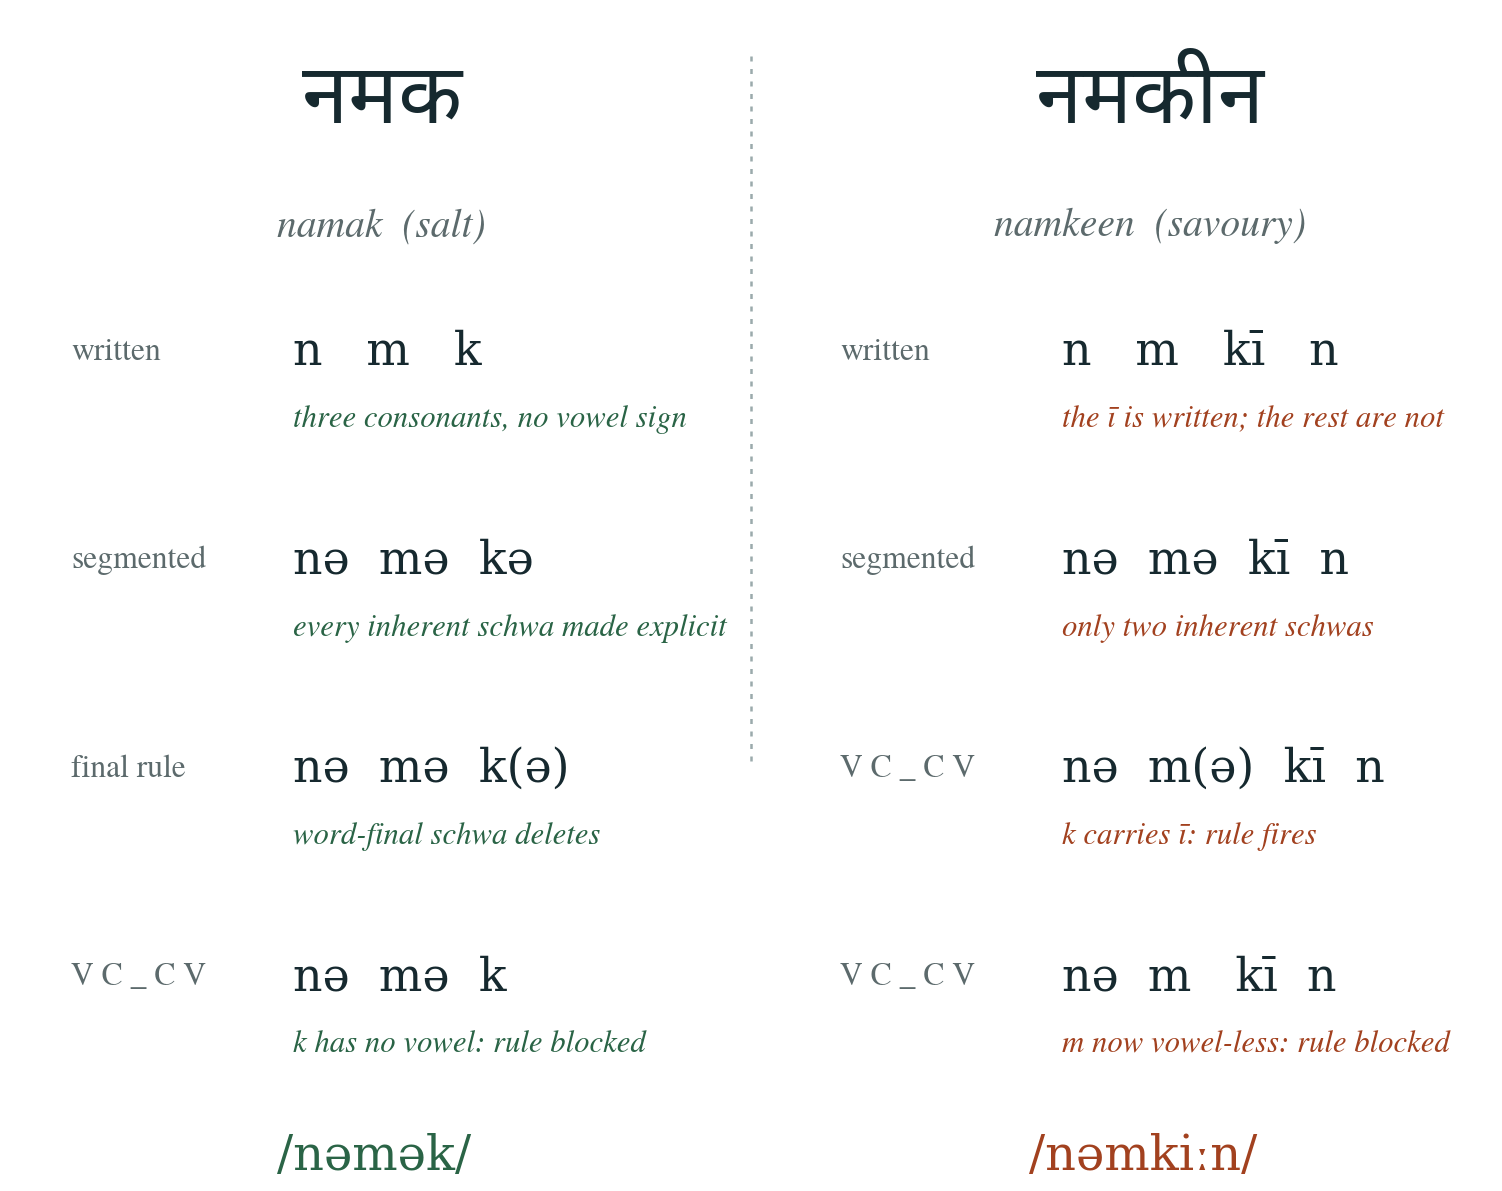
\includegraphics[width=3.85in]{figures/fig_1_1_schwa_derivation.png}
  \caption*{\textbf{Figure 1.2:}  Schwa deletion applied to \dev{नमक} and \dev{नमकीन}. A deleted schwa is shown in brackets. In \dev{नमक} the word-final schwa goes first, which leaves the k with no vowel and blocks the deletion to its left. In \dev{नमकीन} the k already carries a written ī, so the rule fires on the m and then blocks on the n.}
  \addcontentsline{lof}{figure}{Figure 1.2: Schwa deletion applied to \dev{नमक} and \dev{नमकीन}}
\end{figure}

A third example shows why the direction is part of the definition and not a stylistic choice. The word \dev{समझना}, \textit{samajhna}, segments as \ipa{/sə} \ipa{mə} \ipa{dʒʒʱə} \ipa{naː/}. Working from the right, the schwa on the aspirated jha is flanked by a vowel on each side and deletes. That deletion removes the vowel the schwa on the m would have needed on its right, so the m schwa is blocked and survives. The result is \textit{samajhna}. Run the same rule left to right and the m is evaluated while the jha still has its schwa, the pattern matches, and you get \textit{samjhana}, which is not a word anybody says.

Where the rule is known to fail is worth stating now, because it is the reason this project builds a stress-test set rather than a random sample. Compounds and suffixed forms can keep a schwa that the rule deletes, because the morpheme boundary blocks it and the rule has no access to morphology. Perso-Arabic and English borrowings follow the phonotactics of their source language more than they follow Hindi's. And some words simply have two acceptable pronunciations, which is why the elicitation instrument described in Section 3.6 offers speakers a third answer besides yes and no.

Marathi is the other half of the design. It is written in the same script, it shares almost all of Hindi's phone inventory, and it does delete the word-final schwa, but it does not apply the medial rule as a productive process [12]. That one difference is what makes it a control rather than a second target language, and Section 3.7 sets out the reasoning in full.

\subsection*{1.3  Challenges}
\addcontentsline{toc}{subsection}{1.3  Challenges}
With Devanagari underspecifying the vowel, a phonemic front end has to guess more often than one would like, and the guesses are sometimes wrong. Beyond that, the published comparisons very rarely hold anything constant. Two systems usually differ in architecture, data, sampling rate, vocoder and front end all at once, which makes it impossible to attribute a quality gap to any one of them.

The evaluation metrics are easier to get wrong than they look. Mel-cepstral distortion that keeps the zeroth coefficient is partly a measure of loudness rather than of spectral match [14], so a system that is merely quieter scores worse. Pitch error measured on a linear scale is dominated by whichever speaker has the higher pitch, so any average across speakers is skewed. Word error rate loses its meaning unless it is reported next to the recogniser's own error rate on natural ground truth audio [15], and that reference floor is routinely left out.

Cross-lingual evaluation adds a hazard of its own, which is that the tooling is unevenly mature. Forced aligners and speech recognisers are considerably better developed for Hindi than for Marathi [16], so reaching for an automated pipeline risks injecting a tooling difference into a comparison where the language is supposed to be the only thing that changes. Section 4.7.1 describes how this study ended up removing forced alignment for exactly that reason.

\subsection*{1.4  Research Gap}
\addcontentsline{toc}{subsection}{1.4  Research Gap}
We do have strong single-system Indic results, and we also have architectural comparisons for English. What we do not have, and what this research aims to build, is a controlled measurement of how much the front end contributes on a Devanagari language when it is separated from the architecture.

To name the specifics that have been missing: there is no study that holds the architecture, the data, the vocoder, the training budget and the evaluation fixed while varying only the input representation; there is no study that uses a same-script control, which makes it hard to distinguish “Devanagari is hard” from “schwa deletion is hard”; and we found no study that reports how the effect changes with the quantity of training data. Table 1.1 sets the closest existing work against those three requirements.

\begin{table}[htbp]
  \centering
  \small
  \caption*{\textbf{Table 1.1:}  What the closest existing work does and does not hold fixed.}
  \addcontentsline{lot}{table}{Table 1.1: What the closest existing work does and does not hold fixed}
  \begin{tabular}{p{1.82in}p{1.38in}p{1.18in}p{0.93in}}
  \toprule
  \textbf{Work} & \textbf{Isolates the front end} & \textbf{Same-script control} & \textbf{Data-size axis} \\
  \midrule
  Narasimhan et al. [1] & Rule only, no TTS & No & No \\
  Arora et al. [2] & G2P accuracy only & Punjabi, different rule & No \\
  AI4Bharat [8] & No, single system & No & Partly, per language \\
  IndicVoices-R [9] & No, corpus contribution & No & No \\
  MMS [10] & No, one model, 1,000+ languages & No & No \\
  \textbf{This work} & \textbf{Yes, the only variable} & \textbf{Marathi} & \textbf{Five rungs} \\
  \bottomrule
  \end{tabular}
  \par\vspace{3pt}\begin{minipage}{5.95in}\footnotesize\itshape Rows are judged on whether the cited work can answer the question, not on its quality. Each of these papers answers the question it set out to answer.\end{minipage}
\end{table}

\subsection*{1.5  Motivation}
\addcontentsline{toc}{subsection}{1.5  Motivation}
The motivation for this research comes from a very practical question: \textit{2 \{d|बी} G2P or not 2 \dev{बी}?\} Implementing a G2P front end is real work. It means a phone inventory, a normaliser, a schwa implementation, an exception lexicon, and then the maintenance of all four. The fight over whether that work is necessary has two sides, and neither has been given an umpire.

On one side stand the linguistic purists, who insist on a full G2P front end with phonetic inventories and hand tuned schwa deletion rule sets before anything reaches an acoustic model. On the other stand the end-to-end modernists, who feed raw Devanagari characters straight into FastSpeech 2, VITS or Matcha-TTS on the assumption that neural alignment will learn zero duration schwas on its own. What the argument needs is a rigorous study of the exact perceptual, intelligibility and acoustic cost of skipping the front end across modern models. Building the front end for this project took the better part of a month. If current architectures learn schwa deletion from data on their own, that month was wasted and nobody else should spend it. If they do not, the field should stop defaulting to character level input for Indic languages, which is presently common.

\subsection*{1.6  Problem Statement}
\addcontentsline{toc}{subsection}{1.6  Problem Statement}
Holding training budget, evaluation protocol and speaker fixed, does phonemic input from an explicit Devanagari G2P front end improve neural TTS quality in Hindi relative to raw grapheme input? Does the answer depend on the acoustic architecture? Does it survive as training data falls from nine hours to ten minutes? And using Marathi as a same-script control where medial schwa deletion does not apply, is any effect related to schwa deletion rather than to the script in general?

\subsection*{1.7  Research Objectives}
\addcontentsline{toc}{subsection}{1.7  Research Objectives}
\begin{enumerate}[leftmargin=1.9em,itemsep=2pt,topsep=3pt]
  \item Build a speaker-matched, loudness-normalised Hindi and Marathi corpus with frozen, checksummed splits that regenerate identically on any machine.
  \item Implement a Devanagari G2P front end in which schwa deletion is a separately switchable stage, and measure its accuracy against elicited native-speaker judgement before trusting it anywhere downstream.
  \item Train FastSpeech 2, VITS and Matcha-TTS under a provably identical budget, on phonemic and on graphemic input.
  \item Measure the phoneme against grapheme effect across a nested data ladder running from nine hours down to ten minutes.
  \item Repeat the ablation in Marathi in order to separate phonology from script.
  \item Evaluate with verified objective metrics, predicted mean opinion score, a human listening test, and real-time factor measured on consumer hardware.
  \item Release the testbed, the fine-tuned checkpoints and a speaker-validated contested-schwa stress-test set.
\end{enumerate}

\section*{CHAPTER 2  LITERATURE REVIEW}
\addcontentsline{toc}{section}{Chapter 2  Literature Review}
This chapter covers five areas: the acoustic architectures, neural vocoding, how a model obtains its durations, the Indic speech resources this work builds on, and the evaluation methodology. The last section pulls the threads together into the gap that Chapter 1 named.

\subsection*{2.1  Neural Acoustic Models}
\addcontentsline{toc}{subsection}{2.1  Neural Acoustic Models}
Neural text-to-speech has passed through four generative families in about seven years, and the three architectures compared here are drawn one from each of the last three. That is deliberate: a result about the front end that holds across generation paradigms is stronger than one that holds for a single design. The family not represented is the autoregressive one. Tacotron 2 [17] generates one mel frame at a time and learns alignment through attention, which is slow and lets a single attention failure become a skipped or repeated word.

\subsubsection*{2.1.1  FastSpeech 2}
\addcontentsline{toc}{subsubsection}{2.1.1  FastSpeech 2}
FastSpeech 2 [3] is a non-autoregressive transformer of roughly 27 million parameters. A transformer encoder reads the symbol sequence. A variance adaptor then predicts, for every symbol, a duration, a pitch value and an energy value. The length regulator repeats each encoder output as many times as its predicted duration says, which converts a symbol-level sequence into a frame-level one, and a decoder turns that into a mel spectrogram in a single forward pass.

Two consequences follow. Generation is fast and cannot skip or repeat a word, because there is no autoregression to go wrong. But the model is deterministic, so it predicts one duration and one pitch contour where a real speaker produces a sample from a distribution of plausible ones, and averaging over that distribution is heard as flatness. The consequence that matters most here is the duration: FastSpeech 2 needs a duration target from somewhere, and where that target comes from is the subject of Section 2.3.

\begin{figure}[htbp]
  \centering
  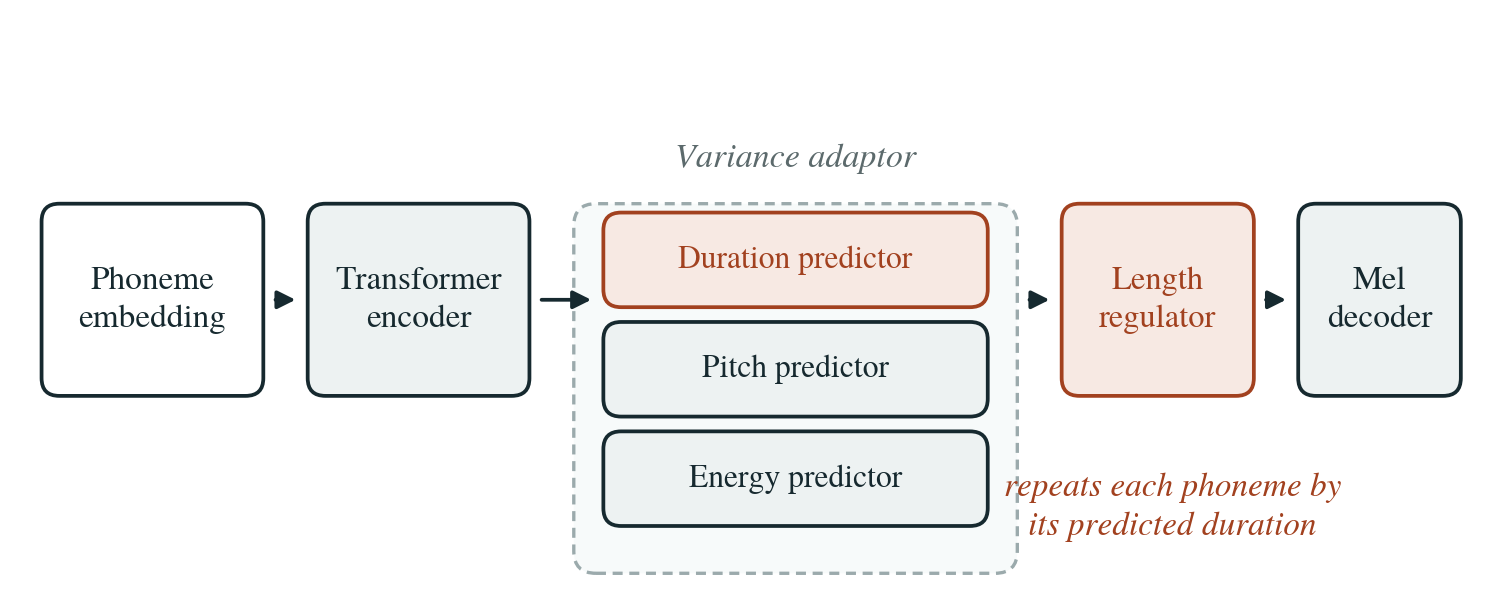
\includegraphics[width=3.85in]{figures/fig_2_1_fastspeech2.png}
  \caption*{\textbf{Figure 2.1:}  FastSpeech 2. The variance adaptor predicts duration, pitch and energy explicitly, and the length regulator uses the duration to expand the symbol sequence to frame rate before a single decoder pass.}
  \addcontentsline{lof}{figure}{Figure 2.1: FastSpeech 2}
\end{figure}

\subsubsection*{2.1.2  VITS}
\addcontentsline{toc}{subsubsection}{2.1.2  VITS}
VITS [4] is the largest of the three at roughly 83 million parameters, and it is the only one that produces a waveform directly with no separate vocoder. Three ideas are stacked on top of each other. A conditional variational autoencoder gives the model a latent representation of the audio. A normalising flow makes the prior over that latent expressive enough to be matched to text, which a simple Gaussian prior would not be. And an adversarial loss on the decoder output pushes the waveform towards realism in the way a vocoder would.

Alignment is found during training by monotonic alignment search, inherited from Glow-TTS [18]. At inference there is no audio to align against, so duration comes from a stochastic duration predictor, which is why two generations of the same sentence differ in rhythm.

One practical fact shapes the experimental design. The MMS release [10] publishes pretrained VITS checkpoints for both Hindi and Marathi, and they are natively 16 kHz. Fine tuning from them is what makes the lower ladder rungs feasible for VITS at all, and the sampling rate they impose is a confound addressed in Section 5.2.

\begin{figure}[htbp]
  \centering
  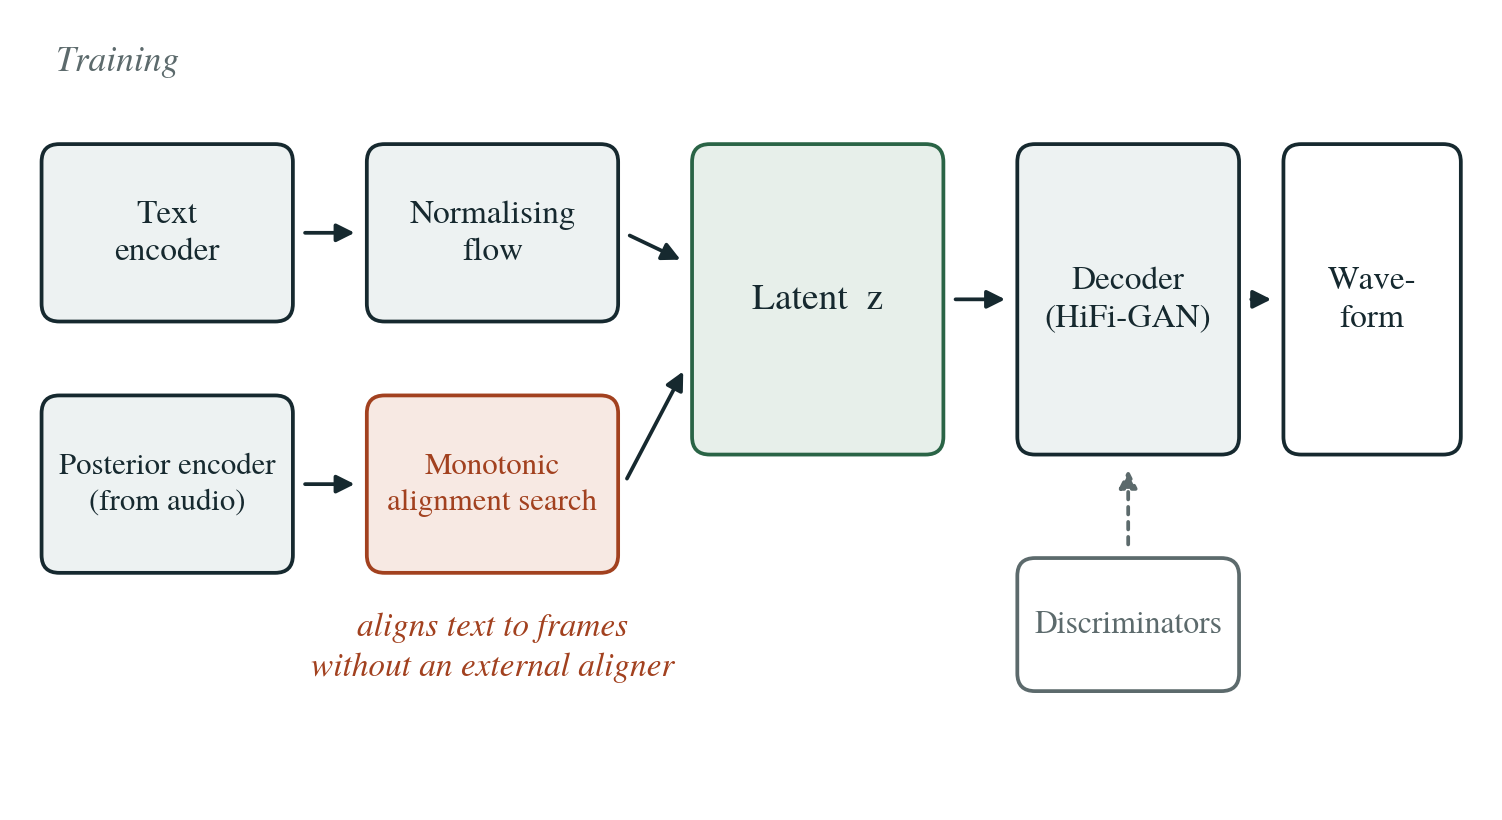
\includegraphics[width=3.85in]{figures/fig_2_2_vits.png}
  \caption*{\textbf{Figure 2.2:}  VITS in training. The posterior encoder reads the audio, the normalising flow makes the text-side prior expressive, monotonic alignment search connects the two, and the decoder with its discriminators produces the waveform. No mel spectrogram is ever a training target.}
  \addcontentsline{lof}{figure}{Figure 2.2: VITS in training}
\end{figure}

\subsubsection*{2.1.3  Matcha-TTS}
\addcontentsline{toc}{subsubsection}{2.1.3  Matcha-TTS}
Matcha-TTS [5] is the smallest of the three at roughly 18 million parameters and also the newest. It is built on optimal-transport conditional flow matching [19]. Rather than learning to remove noise over a long chain of diffusion steps, the model learns a vector field that transports a simple noise distribution to the data distribution, and at inference that field is integrated as an ordinary differential equation. The optimal-transport formulation keeps the transport paths close to straight, and straighter paths can be integrated accurately with fewer solver steps. That is the whole reason an 18 million parameter model reaches diffusion-level quality at a fraction of the inference cost.

Alignment is again monotonic alignment search, so like VITS it needs no external aligner. Matcha-TTS is included because it is the least studied of the three on Indic languages and because its small size makes it the most interesting candidate at the bottom of the data ladder, where an 83 million parameter model has the most to lose.

\begin{figure}[htbp]
  \centering
  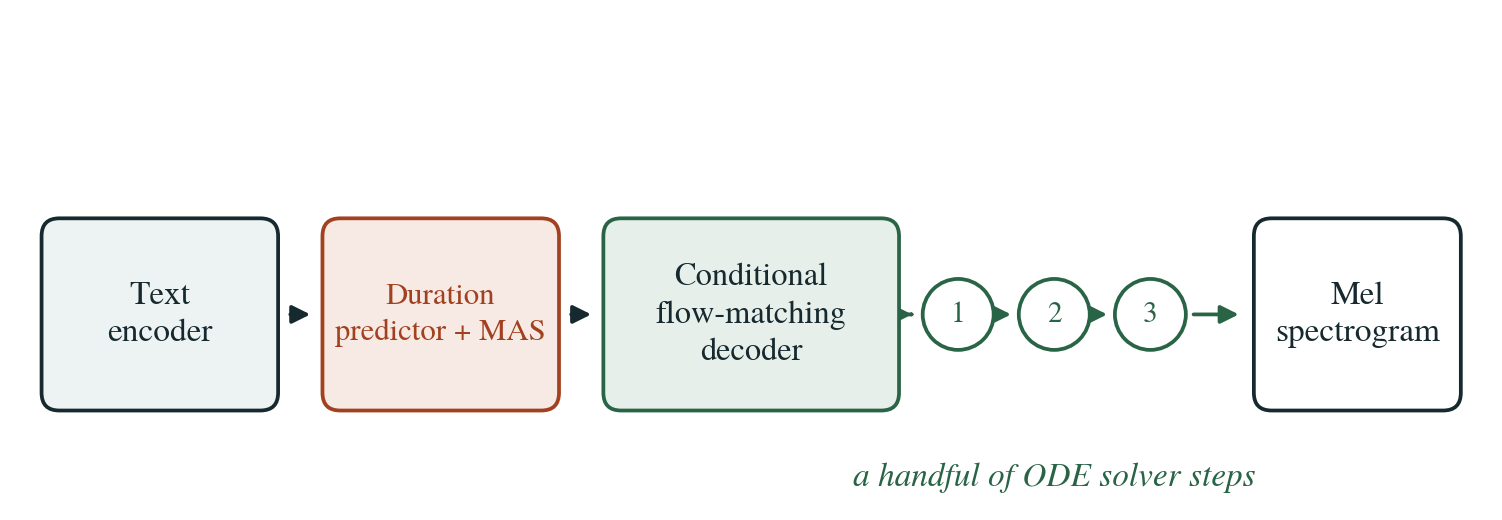
\includegraphics[width=3.85in]{figures/fig_2_3_matcha.png}
  \caption*{\textbf{Figure 2.3:}  Matcha-TTS. The flow-matching decoder is integrated over a small number of ODE solver steps, shown here as the numbered circles, to produce the mel spectrogram.}
  \addcontentsline{lof}{figure}{Figure 2.3: Matcha-TTS}
\end{figure}

\subsubsection*{2.1.4  StyleTTS 2 and Why It Is Not Included}
\addcontentsline{toc}{subsubsection}{2.1.4  StyleTTS 2 and Why It Is Not Included}
StyleTTS 2 [20] reports naturalness above any of the three architectures above, and on some English benchmarks above human recordings. It is excluded from this study for compute rather than for quality. Training it requires a style diffusion model and adversarial training with a large speech language model in the loop, which does not fit inside the budget set out in Section 3.9. Adding it would have cost roughly a third of the total budget and would have bought no new generative paradigm, since the three already chosen cover three. It is listed as future work in Section 6.2.

\subsection*{2.2  Neural Vocoding}
\addcontentsline{toc}{subsection}{2.2  Neural Vocoding}
HiFi-GAN [6] remains the default vocoder and is the one used here. The generator upsamples a mel spectrogram to a waveform through transposed convolutions, with multi-receptive-field fusion blocks so that several kernel sizes and dilation rates observe the signal at once. Two discriminators judge the output. The multi-period discriminator reshapes the one-dimensional waveform into two dimensions at several prime periods, which lets it see the periodic structure of voiced speech that a purely sequential view tends to miss. The multi-scale discriminator looks at the waveform at several downsampling rates and catches the longer-range artefacts.

At around 14 million parameters for the V1 generator, HiFi-GAN is cheap beside the acoustic models, which is why the design holds it fixed across the two systems that need one. If FastSpeech 2 and Matcha-TTS each had their own vocoder, a difference between their outputs could be a difference in vocoder quality rather than in acoustic modelling. VITS bypasses the vocoder entirely, which is an asymmetry inherent to the architecture and is reported as a limitation in Section 5.3.

\begin{figure}[htbp]
  \centering
  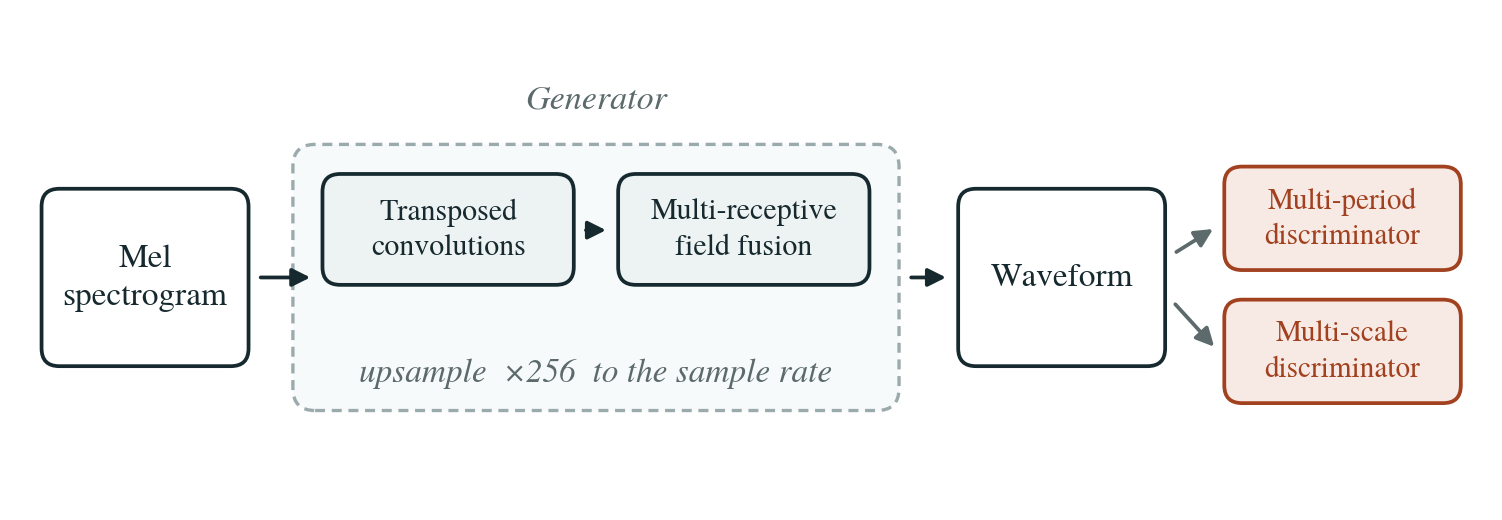
\includegraphics[width=3.85in]{figures/fig_2_4_hifigan.png}
  \caption*{\textbf{Figure 2.4:}  HiFi-GAN. One generator per language is trained on ground-truth mel spectrograms and shared by FastSpeech 2 and Matcha-TTS, so that any difference between them is a difference in acoustic modelling.}
  \addcontentsline{lof}{figure}{Figure 2.4: HiFi-GAN}
\end{figure}

\subsection*{2.3  Where Durations Come From}
\addcontentsline{toc}{subsection}{2.3  Where Durations Come From}
Alignment is the problem of deciding which audio frames belong to which input symbol. Every acoustic model needs an answer, and how a model gets one turns out to be a real difference between the three architectures rather than an implementation detail. Figure 2.5 sets the three approaches side by side.

The traditional answer is external forced alignment: a separate GMM-HMM system such as the Montreal Forced Aligner [16] marks phone boundaries in the training audio, and those boundaries become a supervised duration target. It is accurate, and it is what the original FastSpeech 2 recipe assumed.

The second is monotonic alignment search [18], used by VITS and Matcha-TTS. Dynamic programming finds the monotonic alignment between symbols and frames that maximises likelihood under the model as it currently stands, so the alignment improves as the model does and no external tool is involved.

The third is an internal unsupervised aligner [21], in which a soft attention alignment is learned jointly with the model and sharpened towards a hard monotonic path. The paper shows this matches or beats forced-aligner durations, and it is what current FastSpeech 2 implementations use. That result changed the design of this project, and Section 4.7.1 sets out the three reasons in order.

\begin{figure}[htbp]
  \centering
  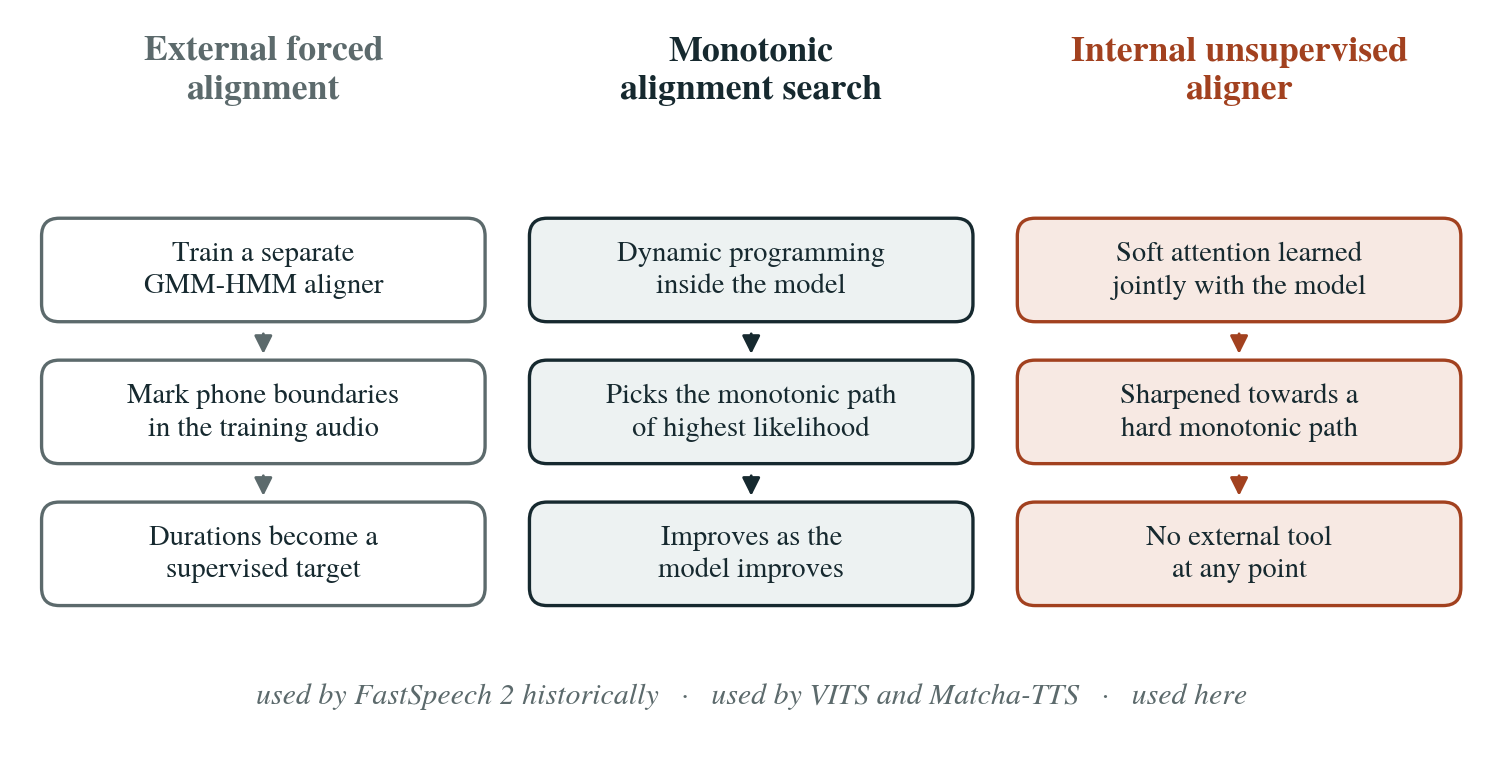
\includegraphics[width=3.85in]{figures/fig_2_5_alignment.png}
  \caption*{\textbf{Figure 2.5:}  Three ways to obtain durations. This study uses the third for FastSpeech 2 and the second for VITS and Matcha-TTS, so that no architecture receives supervision the others do not.}
  \addcontentsline{lof}{figure}{Figure 2.5: Three ways to obtain durations}
\end{figure}

\subsection*{2.4  Devanagari Grapheme-to-Phoneme Conversion}
\addcontentsline{toc}{subsection}{2.4  Devanagari Grapheme-to-Phoneme Conversion}
The rule-based treatment of schwa deletion has been stable since Narasimhan, Sproat and Kiraz [1], whose iterative right-to-left formulation is described in Section 1.2 and implemented in Section 3.5. Arora, Gessler and Schneider [2] revisited the problem as supervised sequence labelling for Hindi and Punjabi and improved on the rule, which establishes both that the rule is not the ceiling and that the remaining errors are learnable. Their work measures G2P accuracy directly; it does not ask what that accuracy is worth once the output reaches a neural acoustic model.

Two further pieces of background are needed for the implementation. The phonology of the two languages follows Ohala [11] for Hindi and Dhongde and Wali [12] for Marathi. The Unicode encoding model for Devanagari [13] carries two traps that produce working programs with silently wrong data, both described in Section 5.1.4.

\subsection*{2.5  Indic Speech Resources}
\addcontentsline{toc}{subsection}{2.5  Indic Speech Resources}
The IIT Madras consortium recordings [7] sit behind most Indian-language TTS work, including both corpora used here. Kumar et al. [8] showed that usable quality is reachable from modest per-language data, which is the empirical basis for believing the lower ladder rungs will produce something worth measuring. IndicVoices-R [9] scaled the resource picture up for synthesis, and MMS [10] supplies the checkpoint the VITS condition initialises from. Between them these papers establish that Indic TTS works and how well. None separates out the contribution of the front end.

\subsection*{2.6  Evaluation Methodology}
\addcontentsline{toc}{subsection}{2.6  Evaluation Methodology}
Mel-cepstral distortion [14] is the standard objective spectral measure and is normally computed after dynamic time warping [22], because a synthesised utterance is not frame-aligned with its reference. Kominek et al. [23] calibrated what a given MCD value means across languages, which is the reason this report treats MCD as a relative measure between systems rather than an absolute one.

Pitch and aperiodicity are conventionally extracted with WORLD [24]; this work uses the probabilistic YIN estimator [25] instead, because it labels frames voiced or unvoiced as part of its output and that labelling is needed for the voiced/unvoiced error rate. Intelligibility is increasingly assessed by transcribing synthesised audio with Whisper [15] and computing word error rate.

Because listening tests are slow, automatic mean opinion score predictors such as UTMOS [26] and NISQA [27] have become common. Both were trained largely on English and Japanese, so this study will measure how well they correlate with its own human ratings and report that as a result. The listening test follows the absolute category rating procedure [28], and loudness normalisation throughout follows ITU-R BS.1770 [29] at the EBU R 128 reference level [30].

\section*{CHAPTER 3  METHODOLOGY}
\addcontentsline{toc}{section}{Chapter 3  Methodology}
\subsection*{3.1  System Design}
\addcontentsline{toc}{subsection}{3.1  System Design}
Figure 3.1 shows the whole arrangement in four rows. Two corpora are standardised and split once. The splits then feed two arms that differ in exactly one respect, which is whether the model sees phonemes or Devanagari characters. Each arm feeds the acoustic architectures, which share one vocoder per language where they need one, and everything is evaluated by the same battery of metrics on the same frozen test set.

\begin{figure}[htbp]
  \centering
  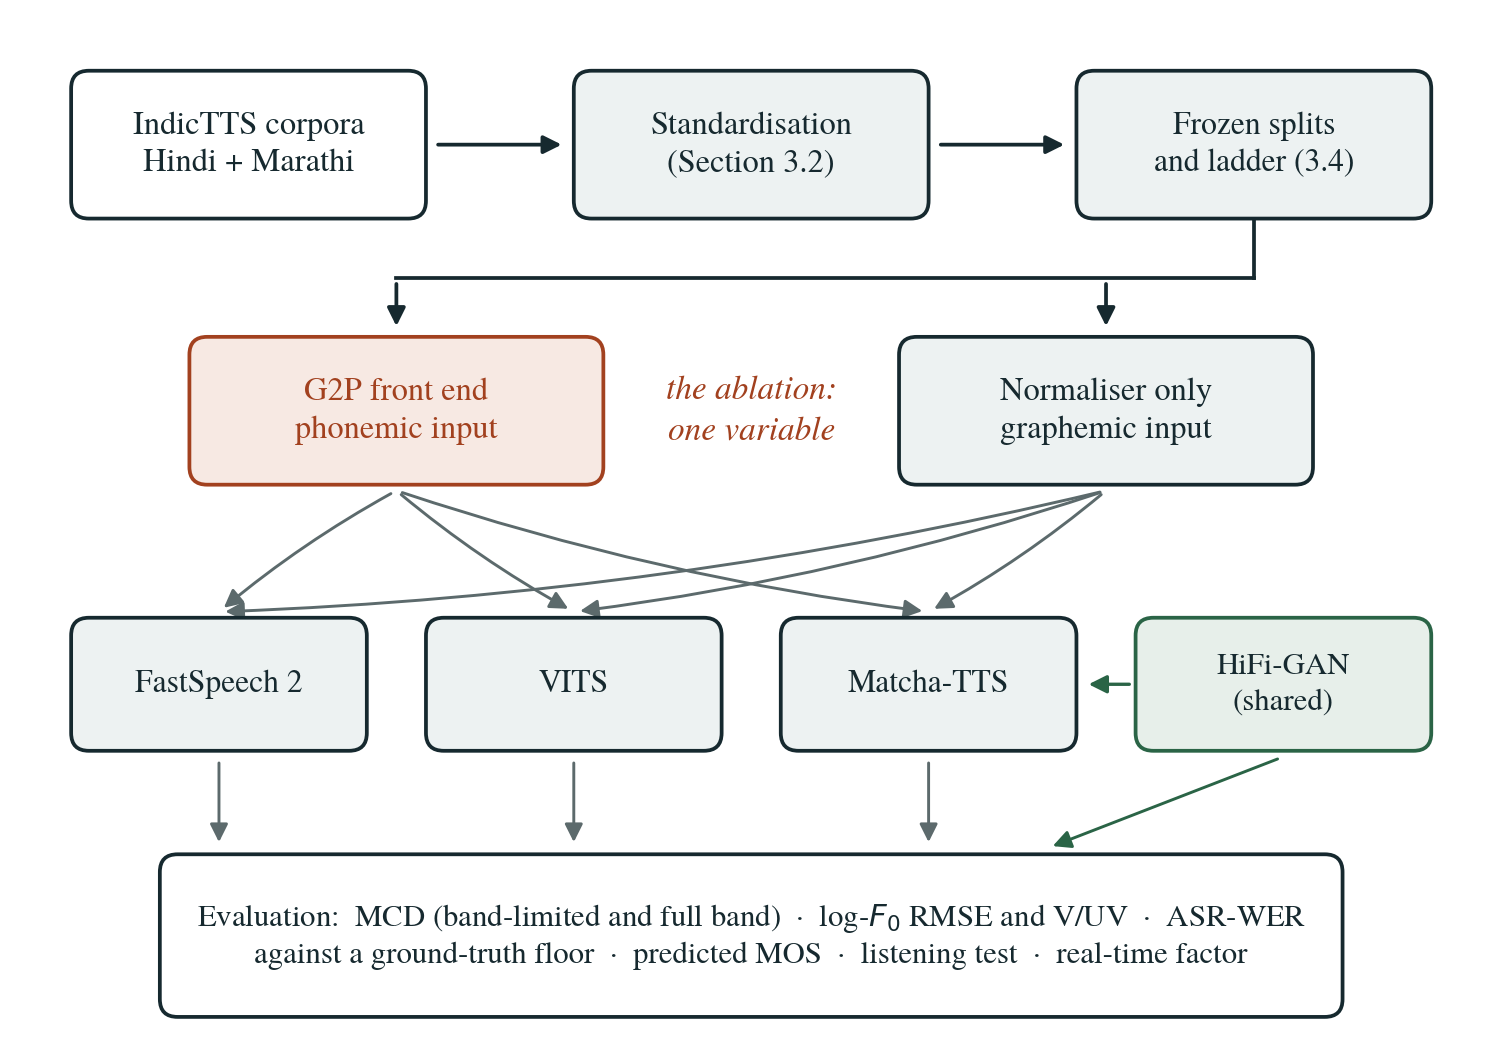
\includegraphics[width=3.85in]{figures/fig_3_1_system.png}
  \caption*{\textbf{Figure 3.1:}  The experimental system. The only difference between the two arms in the second row is the input representation. Everything above and below them is shared.}
  \addcontentsline{lof}{figure}{Figure 3.1: The experimental system}
\end{figure}

\subsection*{3.2  Corpora and Standardisation}
\addcontentsline{toc}{subsection}{3.2  Corpora and Standardisation}
Both corpora come from the SPRING Lab IndicTTS collection, which derives from the IIT Madras consortium recordings [7]. Neither dataset card states the number of hours, the number of speakers or the sampling rate, so all three were measured over the full corpora. An early estimate extrapolated from a 50-utterance sample turned out to be 19 per cent low for Hindi, which is why no figure in this report comes from a sample.

Every utterance then goes through one standardisation chain, shown in Figure 3.2. It is downmixed to mono, silence-trimmed at 40 dB below peak with 50 ms of padding retained at each edge, and normalised to $-23$ LUFS following ITU-R BS.1770 [29] at the EBU R 128 reference level [30]. From there it is resampled twice, to 22.05 kHz for the master and separately to 16 kHz for the VITS arm, and finally peak-guarded at 0.99 to prevent clipping after the gain change.

\begin{figure}[htbp]
  \centering
  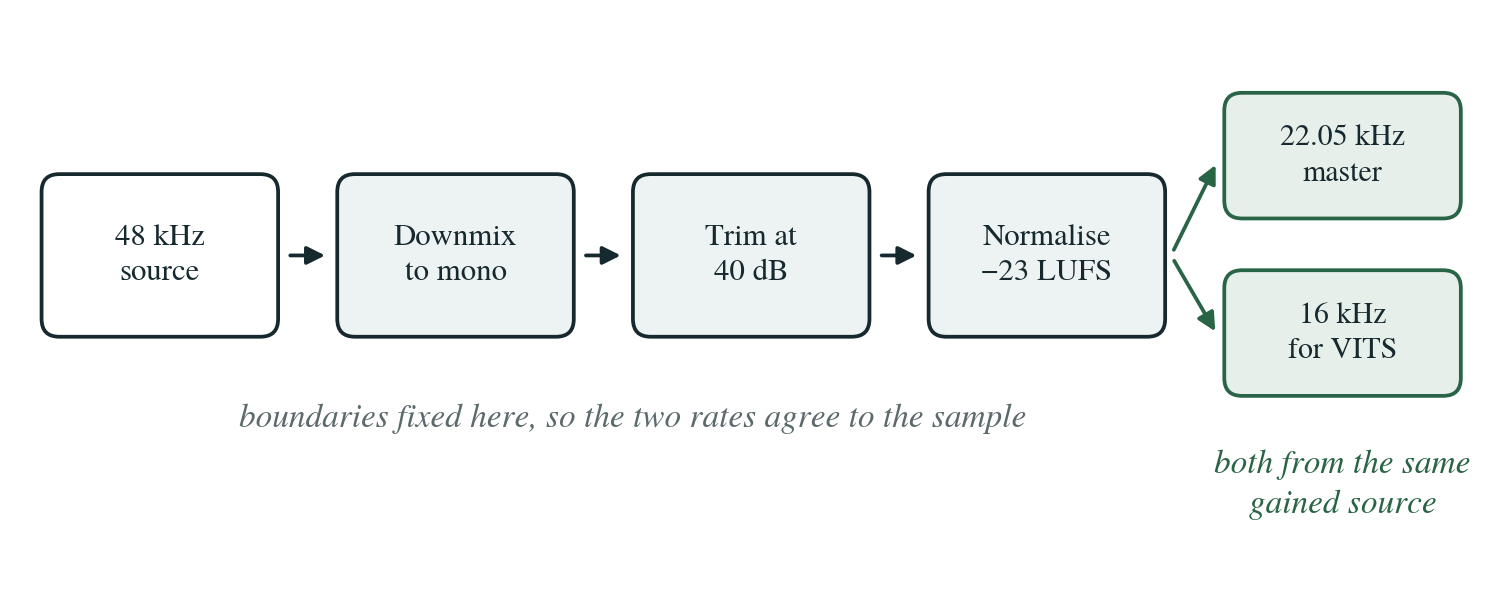
\includegraphics[width=3.85in]{figures/fig_3_2_audio_prep.png}
  \caption*{\textbf{Figure 3.2:}  The audio standardisation chain. Trimming happens at the 48 kHz source and both output rates are derived from the same gained signal.}
  \addcontentsline{lof}{figure}{Figure 3.2: The audio standardisation chain}
\end{figure}

Two details in that chain are deliberate. Trimming happens at the 48 kHz source, so the two output rates share their boundaries to the sample. And the 16 kHz copy is derived from the same gained source rather than from the master, because cascading two resampling operations would put a measurably different signal in front of VITS than the other architectures see, and that difference would surface looking like an architectural effect. Loudness normalisation is used rather than peak normalisation because perceived loudness depends on the whole signal, not on its largest sample.

\subsection*{3.3  Recovering Speaker Identity}
\addcontentsline{toc}{subsection}{3.3  Recovering Speaker Identity}
Both corpora carry a binary field distinguishing two speakers per language, with no key saying which is which. Since the two arms have to be matched on speaker characteristics, the labels were recovered acoustically: median fundamental frequency over 25 sampled utterances per speaker, using the probabilistic YIN estimator [25].

The separation is clean and identical in both languages, as Figure 3.3 shows. The gap is 90.1 Hz in Hindi and 111.5 Hz in Marathi, far wider than any plausible ambiguity around a threshold. Every gender label in this report rests on that measurement and is reported as an inference. The dataset says nothing about it.

\begin{figure}[htbp]
  \centering
  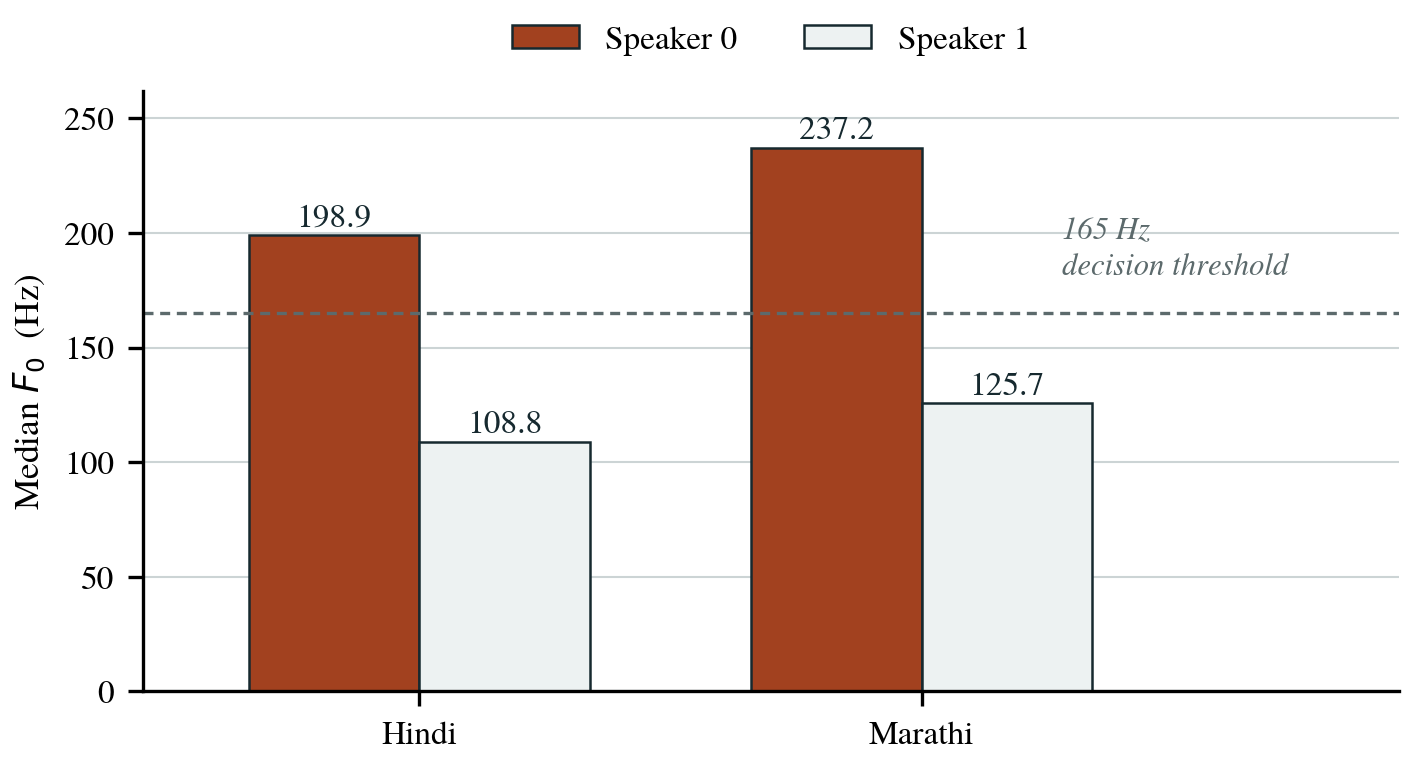
\includegraphics[width=3.85in]{figures/fig_3_3_speaker_f0.png}
  \caption*{\textbf{Figure 3.3:}  Median $F_0$ over 25 sampled utterances per speaker. The dashed line marks the 165 Hz threshold used to assign the labels. Speaker 1 is the lower voice in both languages and is the one this study uses.}
  \addcontentsline{lof}{figure}{Figure 3.3: Median $F_0$ over 25 sampled utterances per speaker}
\end{figure}

The male speaker was selected in both languages. The available hours are near identical either way, so pitch decided it: the two male voices sit 17 Hz apart across the two languages, while the female pair are 38 Hz apart. Matching on the male speakers therefore leaves less acoustic difference between the Hindi and Marathi arms that has nothing to do with schwa deletion.

\subsection*{3.4  Frozen Splits and the Data Ladder}
\addcontentsline{toc}{subsection}{3.4  Frozen Splits and the Data Ladder}
Membership of the test, development and training splits comes from a salted SHA-256 hash of the utterance identifier rather than from a seeded shuffle. A seeded shuffle depends on the order the manifest happened to be written in, so regenerating it elsewhere can hand you a quietly different test set. Hashing the identifier makes membership a property of the utterance, and a rebuild reproduces the test split byte for byte. Three structural properties are asserted on every build: each rung is a strict superset of the rung below, the splits are pairwise disjoint, and no rung reaches outside the training set.

The ladder is the second axis of the study and it is nested rather than independently sampled. Each rung is a prefix of one hash ordering, so every set is contained in the one above it, as Figure 3.4 shows.

\begin{figure}[htbp]
  \centering
  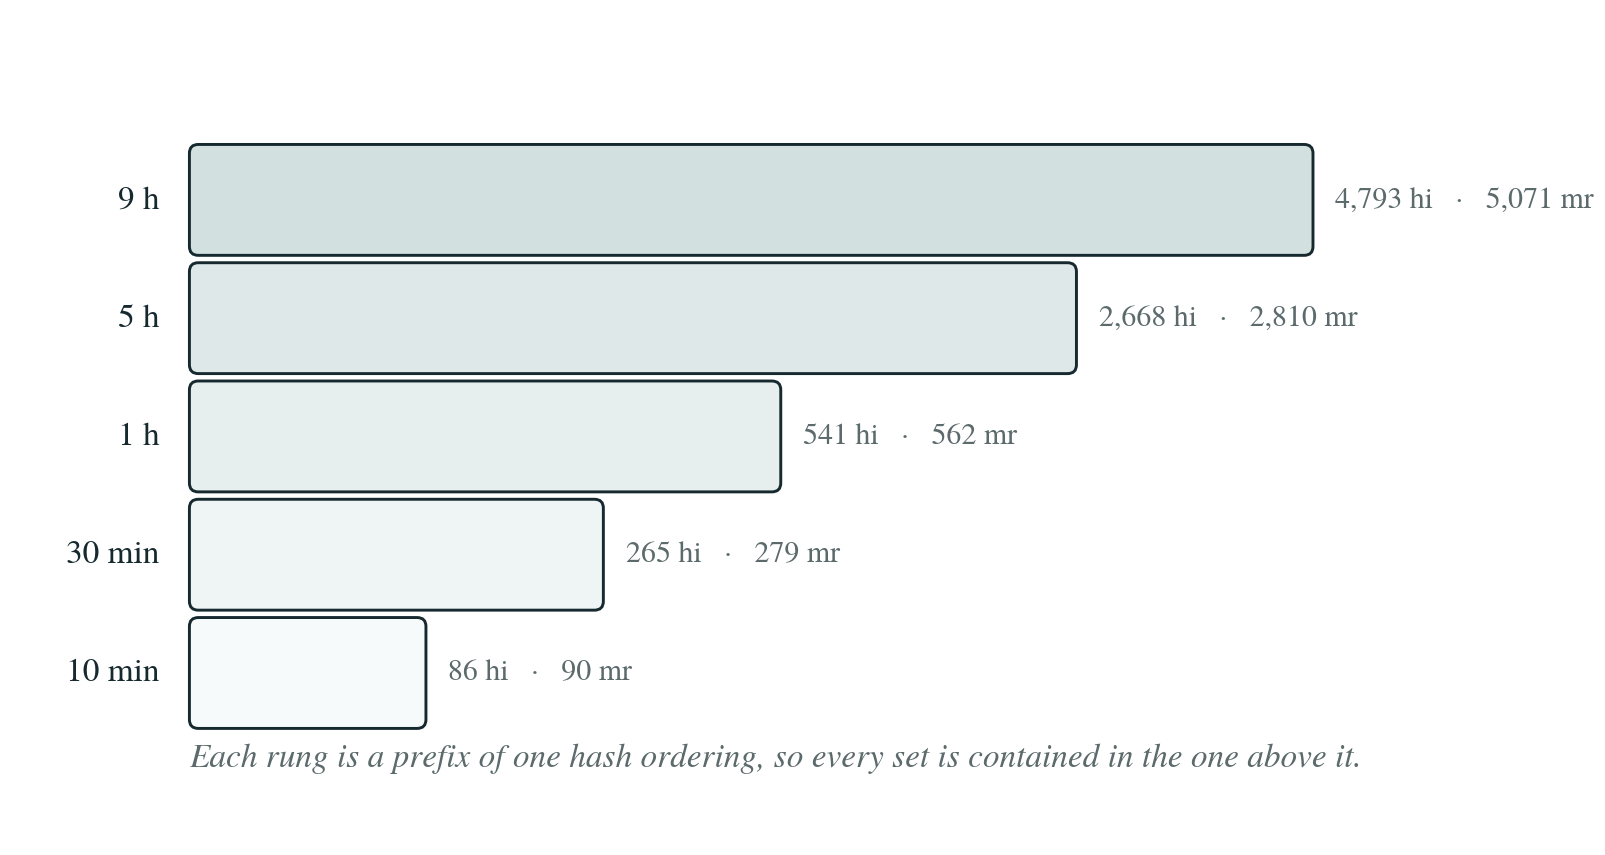
\includegraphics[width=3.85in]{figures/fig_3_4_ladder.png}
  \caption*{\textbf{Figure 3.4:}  The nested data ladder. Utterance counts are given for Hindi and Marathi. Each rung is contained in the one above it, so the only thing that changes between rungs is how much data there is.}
  \addcontentsline{lof}{figure}{Figure 3.4: The nested data ladder}
\end{figure}

Independent sampling would have been easier and would have been wrong. The difference between the one-hour and thirty-minute rungs would then contain both a data-quantity effect and a sampling-variance effect, with no way to separate them, and the data-quantity effect is precisely what the ladder exists to measure.

\subsection*{3.5  The Grapheme-to-Phoneme Front End}
\addcontentsline{toc}{subsection}{3.5  The Grapheme-to-Phoneme Front End}
The front end is built as four separable stages, arranged so that the phonological rule can be switched without touching anything else. That separability is not tidiness for its own sake. It is what makes the control condition a one-line change and the ablation a clean one. Figure 3.5 shows the arrangement.

\begin{figure}[htbp]
  \centering
  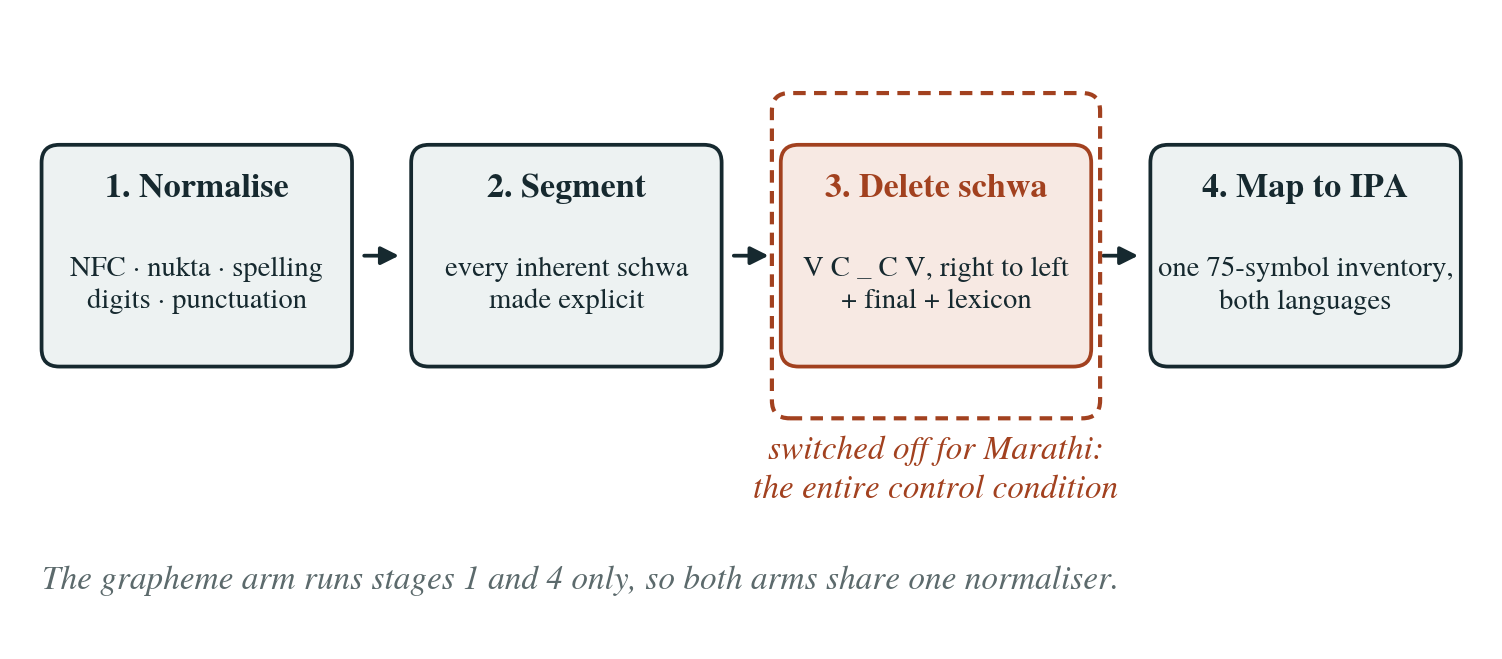
\includegraphics[width=3.85in]{figures/fig_3_5_g2p_pipeline.png}
  \caption*{\textbf{Figure 3.5:}  The four stages of the front end. Stage 3 is switched off for Marathi, and stages 2 and 3 are skipped entirely on the grapheme arm.}
  \addcontentsline{lof}{figure}{Figure 3.5: The four stages of the front end}
\end{figure}

\subsubsection*{3.5.1  Normalisation}
\addcontentsline{toc}{subsubsection}{3.5.1  Normalisation}
The first stage puts the text into a single canonical form. It applies Unicode normalisation form C, composes nukta sequences, repairs a set of corpus spelling slips found by inspection, expands digits into words, and folds punctuation down to four marks.

Two of these need justification. Punctuation is kept rather than stripped, because it is the only prosodic signal the text carries and it appears on roughly one word token in six; it is folded to comma, full stop, question mark and exclamation mark so that rarer marks do not become embedding rows with almost no training signal. Digit expansion is deliberately conservative and raises an exception on anything it cannot expand with certainty, because a wrong number word would be a pronunciation error baked into the training data where nothing downstream would ever check it.

\subsubsection*{3.5.2  Segmentation}
\addcontentsline{toc}{subsubsection}{3.5.2  Segmentation}
The second stage converts the character sequence into segments in which every inherent schwa the abugida implies has been made explicit and tagged as unwritten. This is where the marks of Section 1.2 are resolved: viramas form clusters, matras replace the inherent vowel, the anusvara takes the place of articulation of the following segment, the visarga becomes a voiceless breath, and a matra with no consonant to attach to is dropped with a note recording that it was. Until every schwa is explicit, there is nothing for a deletion rule to operate on.

\subsubsection*{3.5.3  Schwa Deletion}
\addcontentsline{toc}{subsubsection}{3.5.3  Schwa Deletion}
The third stage applies the rule. Figure 3.6 gives it as a flowchart. Word-final deletion runs first and unconditionally. The medial rule then walks the remaining schwas from right to left, deleting any that sit in the context V C \_ C V, and a lexicon of known exceptions is applied at the end so that individual words can override the rule without the rule itself acquiring special cases.

\begin{figure}[htbp]
  \centering
  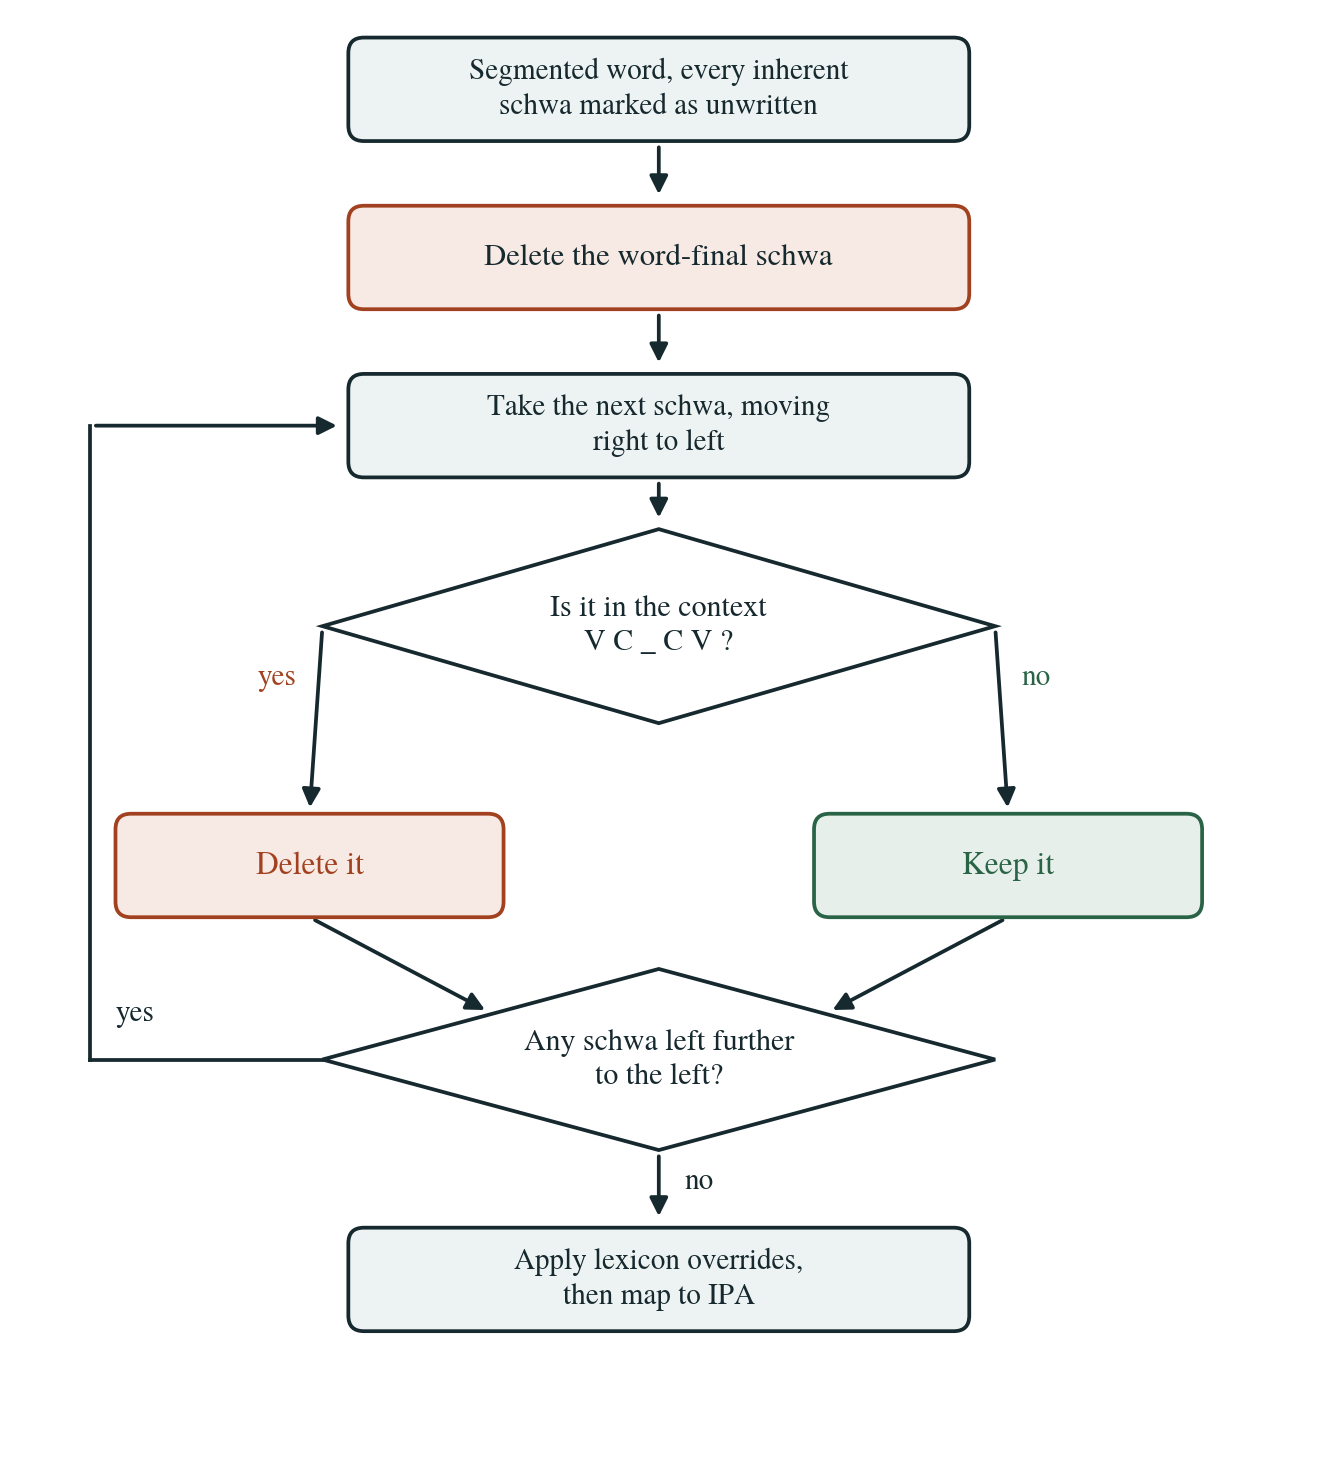
\includegraphics[width=3.85in]{figures/fig_3_6_schwa_algorithm.png}
  \caption*{\textbf{Figure 3.6:}  The schwa deletion stage. The loop back to the top is what makes the rule iterative: each deletion changes the context that the next candidate is evaluated in.}
  \addcontentsline{lof}{figure}{Figure 3.6: The schwa deletion stage}
\end{figure}

Marathi runs this identical code with medial deletion disabled through a single configuration flag, while word-final deletion stays on. That flag is the entire control condition. There is no separate Marathi code path, which means the control comparison cannot be contaminated by an implementation difference between the two languages.

\subsubsection*{3.5.4  Mapping to IPA}
\addcontentsline{toc}{subsubsection}{3.5.4  Mapping to IPA}
The fourth stage maps segments into a single inventory of 75 IPA symbols shared by both languages, following Ohala [11] and Dhongde and Wali [12]. Sharing one inventory lets the two arms occupy one symbol space with no Marathi-only embedding rows, and Section 4.5 reports the measurement confirming the subset relation holds.

\subsubsection*{3.5.5  The Grapheme Arm}
\addcontentsline{toc}{subsubsection}{3.5.5  The Grapheme Arm}
The grapheme arm runs stages 1 and 4 only. It shares the identical normalisation chain and then maps Devanagari characters directly to embedding indices, without segmentation or schwa deletion. Sharing the normaliser is important: if the two arms normalised differently, the ablation would be measuring the normaliser rather than the phonology, and the headline result would be uninterpretable.

\subsection*{3.6  Eliciting Gold Pronunciations}
\addcontentsline{toc}{subsection}{3.6  Eliciting Gold Pronunciations}
The front end has to be validated against something, and that something cannot be written by the person who wrote the rule: gold forms produced by the author would measure the author's consistency with the author's own rule.

The instrument is a sheet that never shows the rule's prediction. Each of the 49 test words appears with its candidate vowels spelled out in place and numbered, as \texttt{n(a1)m(a2)kiin(a3)}, and the speaker marks each slot yes, no or variable. Speakers do not write IPA: asking non-phoneticians to transcribe adds noise unrelated to the question, and the merge step passes their answers through the same converter anyway, so only the judgement is human.

Three design rules follow from a pilot reading that went wrong, described in Section 5.2.3. Every plainly written vowel is stated to be out of scope. Worked examples sit at the top of the sheet, and a check at generation time refuses to write a sheet whose examples appear anywhere in the test set. Items on which speakers disagree are marked variable and reported separately as a variation rate, rather than being resolved by majority.

\subsection*{3.7  Experimental Controls}
\addcontentsline{toc}{subsection}{3.7  Experimental Controls}
The study varies four things and holds everything else fixed. What is varied is the input representation, the architecture, the quantity of training data and the language. Table 3.1 lists what is held constant against what is varied.

\begin{table}[htbp]
  \centering
  \small
  \caption*{\textbf{Table 3.1:}  What is held constant and what is varied.}
  \addcontentsline{lot}{table}{Table 3.1: What is held constant and what is varied}
  \begin{tabular}{p{2.81in}p{2.81in}}
  \toprule
  \textbf{Held constant} & \textbf{Varied} \\
  \midrule
  Training budget: 100,000 steps, 12,000 mel frames per batch, learning rate $2\times10^{-4}$ with inverse-square-root decay after 4,000 warmup steps, fp16, gradient clipping at 1.0 & Input representation: phonemic or graphemic \\
  Speaker: one male voice per language, matched on median $F_0$ & Architecture: FastSpeech 2, VITS, Matcha-TTS \\
  Data: the same frozen, checksummed splits & Training data quantity: five rungs from nine hours to ten minutes \\
  Vocoder: one HiFi-GAN per language, shared & Language: Hindi, with Marathi as the control \\
  Evaluation: the same metrics on the same 300-utterance test set &  \\
  \bottomrule
  \end{tabular}
\end{table}

The budget line is the study's central claim, so it is enforced by an assertion rather than by recollection. A function compares every budget field across all acoustic runs each time the seventeen configuration files are generated and refuses to write them if any differ. A second assertion refuses two runs whose settings hash identically under different identifiers; Section 5.1.2 reports what it caught the first time it ran.

The control logic is worth stating explicitly, because it is what the Marathi arm buys. Figure 3.7 gives the four possible outcomes and what each one would mean.

\begin{figure}[htbp]
  \centering
  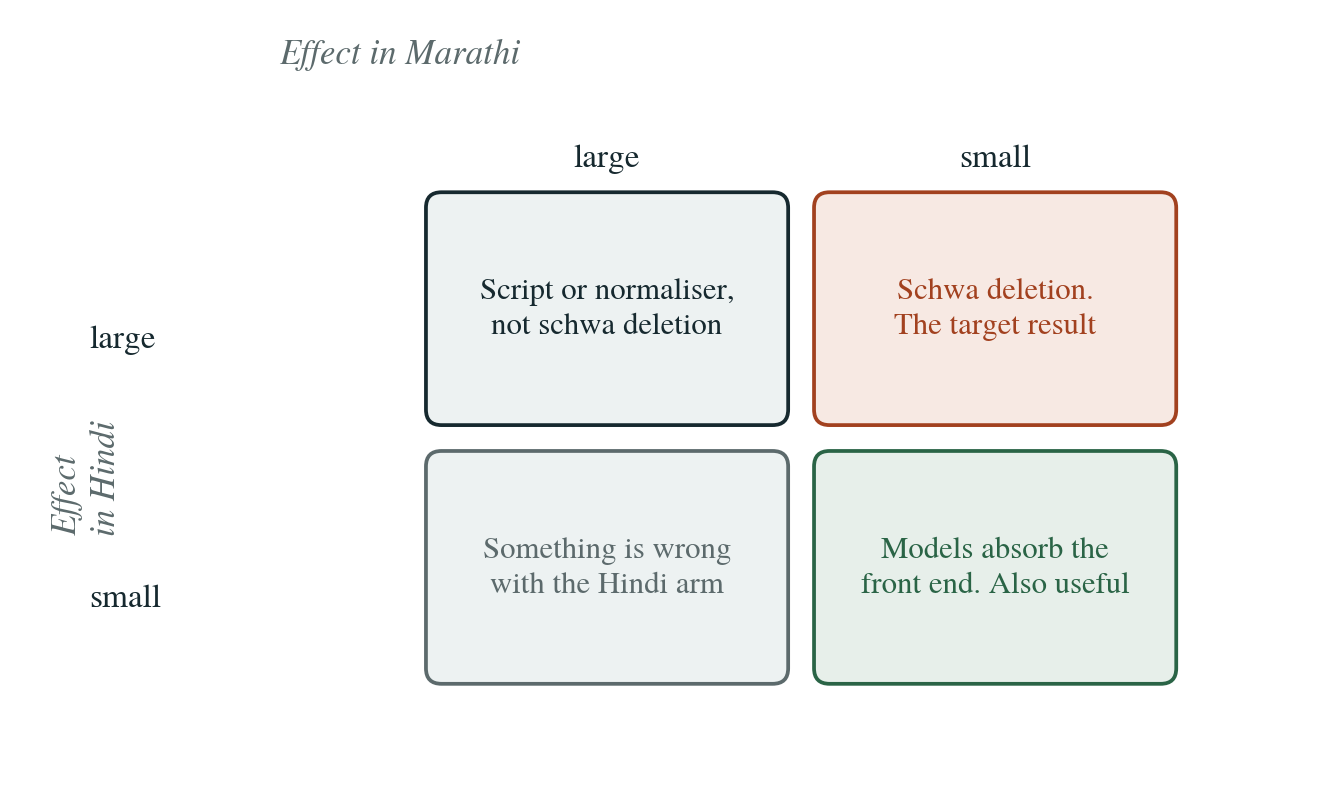
\includegraphics[width=3.85in]{figures/fig_3_7_control_logic.png}
  \caption*{\textbf{Figure 3.7:}  The control logic. A large effect in Hindi together with a small one in Marathi is the outcome the design exists to detect, because Marathi has the same script but not the medial rule.}
  \addcontentsline{lof}{figure}{Figure 3.7: The control logic}
\end{figure}

No other pairing gives this cleanly. Hindi against English would change the script, the phonology, the corpus and the resource level at once. Marathi changes the rule and holds the rest.

\subsection*{3.8  Evaluation Metrics}
\addcontentsline{toc}{subsection}{3.8  Evaluation Metrics}
A metric that is only ever exercised on real audio tends to be wrong in ways nobody notices until a reviewer asks. Both of the implemented objective metrics were therefore checked against answers that can be derived on paper, and Section 4.6 reports those checks.

\subsubsection*{3.8.1  Mel-Cepstral Distortion}
\addcontentsline{toc}{subsubsection}{3.8.1  Mel-Cepstral Distortion}
MCD [14] measures the distance between two mel cepstra frame by frame. The mel cepstrum comes from taking the logarithm of the mel filterbank energies and applying a discrete cosine transform, which packs the spectral envelope into the low-order coefficients. The distortion is

\begin{equation*}
  \mathrm{MCD} \;=\; \frac{10\sqrt{2}}{\ln 10}\;
  \sqrt{\sum_{d=1}^{24}\bigl(c_d-\hat{c}_d\bigr)^{2}}
\end{equation*}

averaged over aligned frames. The constant evaluates to 6.1419 and converts the natural-log cepstral distance into decibels. This implementation uses 24 coefficients and excludes the zeroth, and aligns the two sequences with dynamic time warping [22] before computing the distance.

Both choices carry an argument. The zeroth coefficient is the mean of the log mel energies, which is overall loudness, so keeping it would make MCD partly a measure of gain. Dropping it makes the measure blind to gain, and the reason is exact: scaling a waveform multiplies its power spectrum by a constant, which in the log domain is a constant offset across every mel band, and a constant vector has energy only in the zeroth DCT coefficient.

The alignment matters for a different reason. A model with an explicit duration predictor differs systematically in timing from an end-to-end one, and a frame-aligned comparison would charge that timing difference as spectral error. Warping first separates the two. Figure 3.8 illustrates both points.

\begin{figure}[htbp]
  \centering
  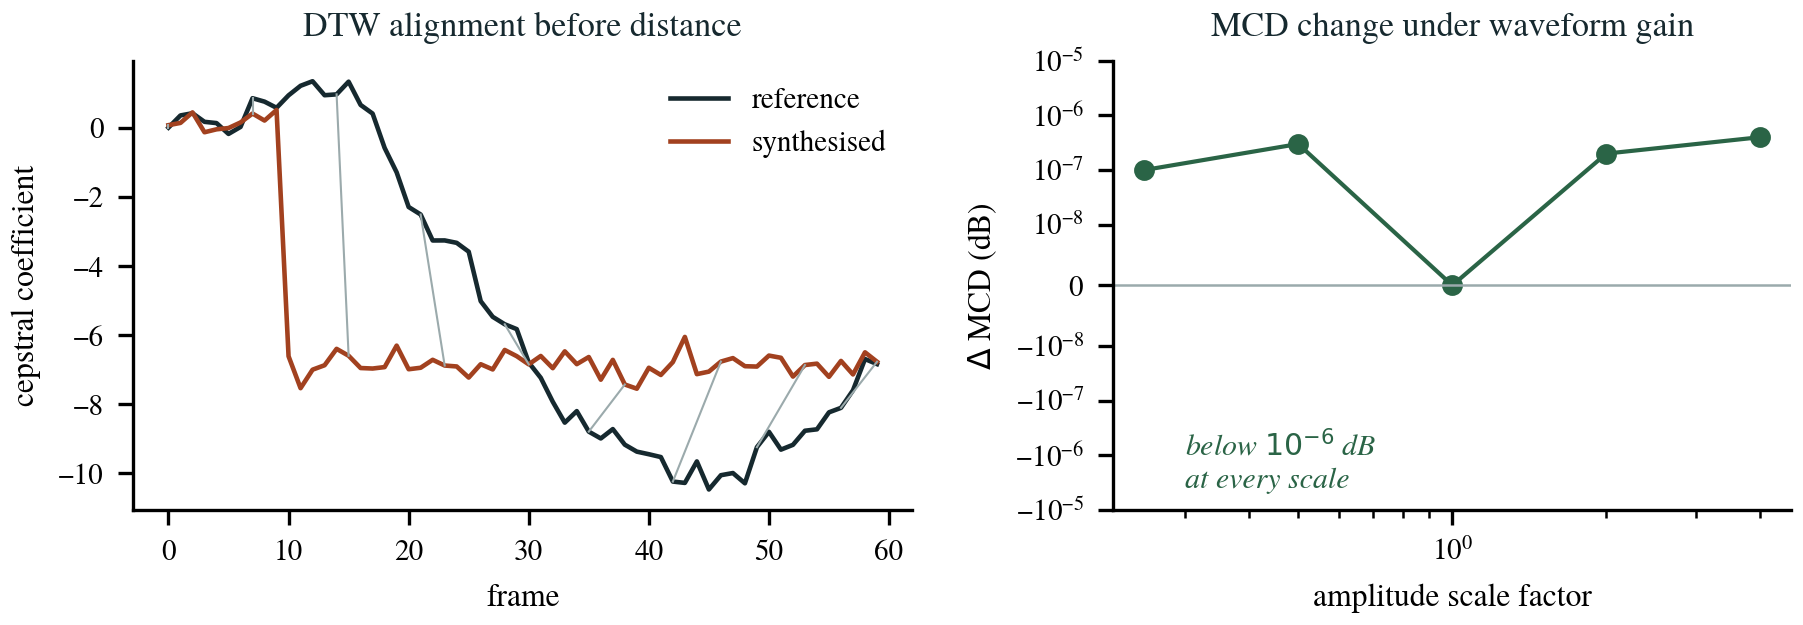
\includegraphics[width=3.85in]{figures/fig_3_8_mcd_dtw.png}
  \caption*{\textbf{Figure 3.8:}  Left, dynamic time warping aligns the synthesised and reference trajectories before any distance is computed. Right, the measured change in MCD when the input waveform is scaled, which stays below $10^{-6}$ dB at every scale factor tested.}
  \addcontentsline{lof}{figure}{Figure 3.8: Left, dynamic time warping aligns the synthesised and reference trajectories before any distance is computed}
\end{figure}

\subsubsection*{3.8.2  Pitch and Voicing Error}
\addcontentsline{toc}{subsubsection}{3.8.2  Pitch and Voicing Error}
Fundamental frequency is extracted with the probabilistic YIN estimator [25] over a 60 to 500 Hz range, which also labels every frame voiced or unvoiced. The error is computed in the natural logarithm domain over the frames that both signals agree are voiced.

The logarithm is not cosmetic. Pitch perception is ratio based, so a ten per cent error is the same perceptual error at 100 Hz and at 300 Hz. A linear root mean square error would call it 10 Hz on one voice and 30 Hz on the other, and any average across speakers would then be dominated by the lower-pitched one.

Prosody is reported as two numbers rather than one. Alongside the pitch error, the voiced against unvoiced error rate records how often the two signals disagree about whether a frame is voiced at all. A system with correct voicing and wrong pitch has a different defect from one with the reverse, and a single combined number would hide which of the two had gone wrong.

Two guards are built in and both are tested. Mismatched track lengths raise rather than truncate to the shorter, because truncation would favour a system predicting shorter durations: the part it got wrong would never be scored. And a comparison with no commonly voiced frames returns not-a-number rather than zero, so an utterance rendered as silence cannot be recorded as a perfect score.

\subsubsection*{3.8.3  Intelligibility}
\addcontentsline{toc}{subsubsection}{3.8.3  Intelligibility}
Synthesised audio is transcribed with Whisper [15] and word error rate is computed against the text that was synthesised. This measures the one thing MCD cannot see, which is whether the utterance says the right words, and a schwa in the wrong place is exactly that kind of error.

The absolute number is meaningless on its own, because the recogniser has its own error rate on real speech. The same recogniser is therefore run over the ground-truth test audio first, and synthesised word error rate is reported relative to that floor. Without it there is no way to separate a poor synthesiser from a poor recogniser.

\subsubsection*{3.8.4  Predicted and Human Mean Opinion Score}
\addcontentsline{toc}{subsubsection}{3.8.4  Predicted and Human Mean Opinion Score}
UTMOS [26] and NISQA [27] are run over every test utterance to give a predicted mean opinion score. They are cheap and cover the whole test set, and they are reported as predicted rather than as MOS, for the reason given in Section 2.6.

The human listening test settles subjective claims. It follows the absolute category rating procedure [28] with ground-truth audio as an anchor, and the stimulus set is chosen to include the contested-schwa items rather than drawn at random, since those are where a front-end difference should be audible if it is audible anywhere. Every stimulus is low-pass filtered to 8 kHz so that all systems are heard at equal bandwidth.

\subsubsection*{3.8.5  Real-Time Factor}
\addcontentsline{toc}{subsubsection}{3.8.5  Real-Time Factor}
Real-time factor is generation time divided by the duration of the audio generated, measured on consumer hardware rather than on the training accelerator. A practitioner choosing an architecture for a low-resource language cares about deployment cost, and the three architectures differ by more than a factor of four in parameter count.

\subsection*{3.9  Reproducibility and Compute}
\addcontentsline{toc}{subsection}{3.9  Reproducibility and Compute}
One YAML file defines one training run, and it carries a hash over every field that affects the trained model. A results row records its run identifier and that hash, so any number appearing in the final paper traces back to the exact settings that produced it. The run identifier is deliberately excluded from the hash, for a reason Section 5.2 explains.

Corpus preparation, the front end and the evaluation code run locally on an Apple M5. Training is planned on free-tier GPU resources capped at 30 GPU-hours a week in 12-hour sessions. That session limit is where the checkpoint-resume requirement comes from: without a verified resume path a killed session costs a whole run. Verification pushes a checkpoint to a remote store, deletes it locally, pulls it back and compares SHA-256 digests, because an untested resume path is not a safety net.

\section*{CHAPTER 4  RESULTS}
\addcontentsline{toc}{section}{Chapter 4  Results}
Nothing has been trained yet, so everything in this chapter is a property of the corpus, the front end or the measuring apparatus. Each had to be established before any model was trained, because a defect in any of them would have propagated into every result that followed. Several turned out to be findings in their own right, and those are discussed in Chapter 5.

\subsection*{4.1  Corpus Profile}
\addcontentsline{toc}{subsection}{4.1  Corpus Profile}
Table 4.1 gives the measured properties of both corpora. All of it was measured over the full set of files. The gender column is an inference from median fundamental frequency, as described in Section 3.3, and not a dataset label.

\begin{table}[htbp]
  \centering
  \small
  \caption*{\textbf{Table 4.1:}  Measured corpus properties. Gender is inferred from median $F_0$.}
  \addcontentsline{lot}{table}{Table 4.1: Measured corpus properties. Gender is inferred from median $F_0$}
  \begin{tabular}{p{1.33in}>{\raggedleft\arraybackslash}p{0.98in}>{\raggedleft\arraybackslash}p{0.98in}>{\raggedleft\arraybackslash}p{0.98in}>{\raggedleft\arraybackslash}p{0.88in}}
  \toprule
  \textbf{} & \textbf{Hindi sp. 0} & \textbf{Hindi sp. 1} & \textbf{Marathi sp. 0} & \textbf{Marathi sp. 1} \\
  \midrule
  Utterances & 5,983 & 5,842 & 5,362 & 5,577 \\
  Hours (raw) & 13.10 & 13.13 & 11.49 & 10.88 \\
  Median $F_0$ (Hz) & 198.9 & 108.8 & 237.2 & 125.7 \\
  Inferred gender & female & male & female & male \\
  \textbf{Corpus total} & \textbf{11,825 utts, 26.23 h, 48 kHz} &  & \textbf{10,939 utts, 22.37 h, 48 kHz} &  \\
  \bottomrule
  \end{tabular}
\end{table}

The first estimate of these hours came from a 50-utterance sample and gave 21.99 hours for Hindi against the 26.23 measured over the full corpus, an error of 19 per cent. Marathi was closer, at 22.97 against 22.37. The Hindi sample was simply not representative, which is why the full pass was run and why no figure in this report is extrapolated.

Transcript quality was checked using characters per second of audio, on the reasoning that a transcript belonging to different audio would appear as an outlier on that measure. The Hindi median is 12.52 characters per second (p1 9.16, p99 15.77) and Marathi sits at 9.10 (6.64, 11.70). Nothing in either corpus falls outside 0.4 to 2.0 times its median, so there were no misaligned transcripts to clean. The longest Hindi utterance runs 127.7 seconds and was assumed to be corrupt until it was checked: at 1,600 characters that is 12.5 characters per second, exactly the corpus median. It is a long read, not a broken row.

\subsection*{4.2  Standardisation Outcomes}
\addcontentsline{toc}{subsection}{4.2  Standardisation Outcomes}
Table 4.2 reports what came out of the standardisation chain for the selected male speaker in each language, under a length filter of 1 to 15 seconds.

\begin{table}[htbp]
  \centering
  \small
  \caption*{\textbf{Table 4.2:}  Standardised corpora, male speaker, 1 to 15 s, $-23$ LUFS.}
  \addcontentsline{lot}{table}{Table 4.2: Standardised corpora, male speaker, 1 to 15 s, $-23$ LUFS}
  \begin{tabular}{p{2.42in}>{\raggedleft\arraybackslash}p{1.53in}>{\raggedleft\arraybackslash}p{1.53in}}
  \toprule
  \textbf{} & \textbf{Hindi} & \textbf{Marathi} \\
  \midrule
  Utterances retained & 5,485 & 5,559 \\
  Hours & 10.289 & 9.884 \\
  Hours before trimming & 10.887 & 10.795 \\
  Loss to silence trimming & 5.5\% & 8.4\% \\
  Utterances hitting the peak guard & 1 & 0 \\
  Gain range applied & $-8.7$ to +2.1 dB & $-9.2$ to +2.8 dB \\
  \bottomrule
  \end{tabular}
\end{table}

The length filter was set at 1 to 15 seconds rather than the 1 to 12 originally planned, and the reason is visible in Table 4.3. At 1 to 12 seconds no single Hindi speaker reaches a ten-hour top rung. At 1 to 15 seconds every candidate speaker clears it. Fifteen seconds at 22.05 kHz with a hop of 256 samples is 1,292 mel frames, which all three architectures handle comfortably.

\begin{table}[htbp]
  \centering
  \small
  \caption*{\textbf{Table 4.3:}  Available hours per speaker under three length filters.}
  \addcontentsline{lot}{table}{Table 4.3: Available hours per speaker under three length filters}
  \begin{tabular}{p{1.92in}>{\raggedleft\arraybackslash}p{1.13in}>{\raggedleft\arraybackslash}p{1.13in}>{\raggedleft\arraybackslash}p{1.13in}}
  \toprule
  \textbf{Speaker} & \textbf{1 to 12 s} & \textbf{1 to 15 s} & \textbf{1 to 20 s} \\
  \midrule
  Hindi female & 9.05 & 10.73 & 11.84 \\
  Hindi male & 8.96 & 10.89 & 11.93 \\
  Marathi female & 10.09 & 11.19 & 11.48 \\
  Marathi male & 10.18 & 10.80 & 10.87 \\
  \bottomrule
  \end{tabular}
\end{table}

\subsection*{4.3  Frozen Splits and the Data Ladder}
\addcontentsline{toc}{subsection}{4.3  Frozen Splits and the Data Ladder}
Silence trimming cost more than the original plan assumed, and that had a consequence which had not been planned for. After trimming, and after the frozen test and development sets are taken out, only 9.53 hours of Hindi and 9.16 hours of Marathi training audio survive. The ladder was going to start at ten hours. It now starts at nine, because matching the rungs across the two languages matters more than a round number: an unmatched top rung would drop a data-quantity difference into the control comparison, which is the one place it must not be.

\begin{table}[htbp]
  \centering
  \footnotesize
  \caption*{\textbf{Table 4.4:}  Frozen splits and the nested data ladder, in utterances.}
  \addcontentsline{lot}{table}{Table 4.4: Frozen splits and the nested data ladder, in utterances}
  \begin{tabular}{p{0.70in}>{\raggedleft\arraybackslash}p{0.40in}>{\raggedleft\arraybackslash}p{0.37in}>{\raggedleft\arraybackslash}p{0.55in}>{\raggedleft\arraybackslash}p{0.49in}>{\raggedleft\arraybackslash}p{0.49in}>{\raggedleft\arraybackslash}p{0.40in}>{\raggedleft\arraybackslash}p{0.55in}>{\raggedleft\arraybackslash}p{0.55in}}
  \toprule
  \textbf{} & \textbf{Test} & \textbf{Dev} & \textbf{Train} & \textbf{9 h} & \textbf{5 h} & \textbf{1 h} & \textbf{30 min} & \textbf{10 min} \\
  \midrule
  Hindi & 300 & 100 & 5,085 & 4,793 & 2,668 & 541 & 265 & 86 \\
  Marathi & 300 & 100 & 5,159 & 5,071 & 2,810 & 562 & 279 & 90 \\
  \bottomrule
  \end{tabular}
  \par\vspace{3pt}\begin{minipage}{5.95in}\footnotesize\itshape Hindi train is 9.525 h and test 0.579 h; Marathi train is 9.160 h and test 0.542 h.\end{minipage}
\end{table}

All three structural assertions pass. Every ladder rung is a strict superset of the rung below it, the three splits are pairwise disjoint, and no rung reaches outside the training set. Rebuilding the splits from scratch reproduces the test file byte for byte, which is the property the hash-based membership was chosen for.

\subsection*{4.4  Grapheme-to-Phoneme Coverage}
\addcontentsline{toc}{subsection}{4.4  Grapheme-to-Phoneme Coverage}
The front end was developed against 49 hand-picked words and handled all of them. It was then run over all 11,044 corpus transcripts, and 4.1 per cent of Hindi phone tokens and 2.7 per cent of Marathi turned out to have no mapping at all. Both figures are now zero, as Table 4.5 shows.

\begin{table}[htbp]
  \centering
  \small
  \caption*{\textbf{Table 4.5:}  Coverage over both corpora after correction.}
  \addcontentsline{lot}{table}{Table 4.5: Coverage over both corpora after correction}
  \begin{tabular}{p{2.42in}>{\raggedleft\arraybackslash}p{1.53in}>{\raggedleft\arraybackslash}p{1.53in}}
  \toprule
  \textbf{} & \textbf{Hindi} & \textbf{Marathi} \\
  \midrule
  Word tokens & 99,958 & 55,492 \\
  Phone tokens & 494,863 & 375,684 \\
  Unknown symbols & 0 & 0 \\
  Inventory used of 75 declared & 72 & 67 \\
  \bottomrule
  \end{tabular}
\end{table}

Getting to zero meant fixing seven classes of problem a curated test set was never going to surface. Nine Hindi tokens carried a nukta on a consonant that has no nukta form, and the stray mark also broke the parse of the character after it. One hundred and ninety-nine Marathi tokens were the letter RRA. There were keyboard slips producing an invalid candra-O sequence, and a colon typed inside a word where a visarga belonged. The OM ligature is a syllable written as one letter and needed expanding. Southern short vowels appeared that neither language distinguishes. And some vowel signs had no consonant to attach to.

\subsection*{4.5  The Shared Phone Inventory}
\addcontentsline{toc}{subsection}{4.5  The Shared Phone Inventory}
Marathi's inventory turns out to be a strict subset of Hindi's, lacking five symbols that are all Perso-Arabic or otherwise marginal. This was measured over all 11,044 transcripts, not assumed, and it is what lets the two arms share one symbol table with no Marathi-only embedding rows.

One weakness belongs in the same place. Three Marathi phones occur fewer than three times in the entire corpus, so those embedding rows will receive essentially no gradient. Merging the nukta consonants for Marathi is the obvious mitigation and has been left as a training configuration decision rather than applied silently, so that the choice stays visible in the run configuration.

\subsection*{4.6  Metric Verification}
\addcontentsline{toc}{subsection}{4.6  Metric Verification}
Both objective metrics were checked against answers that can be derived on paper. Running them over real audio and observing that nothing crashed would not have shown that either was correct.

MCD proved amplitude invariant. Scaling the input waveform by 0.25 changes the computed value by less than $10^{-6}$ dB, which is the property predicted by the argument in Section 3.8.1. If that test ever failed, every MCD figure in the study would be partly a loudness measurement and nothing in the results would show it.

Log-$F_0$ root mean square error reports ln(1.1) for a ten per cent pitch error at 100 Hz and again at 300 Hz, exact to $10^{-12}$. Both guards described in Section 3.8.2 are tested and both behave. The test suite stands at 78 tests, all passing on both the development machine and in the container.

One figure in this chapter is explicitly not a result. Scoring the schwa rule against the 49-item gold set returns 49 out of 49, which measures the consistency of the implementation with gold forms written by the same author in the same sitting. The scorer refuses to report a validated figure until independent speakers have checked the items, and that pass is still outstanding.

\subsection*{4.7  Revised Design Decisions}
\addcontentsline{toc}{subsection}{4.7  Revised Design Decisions}
Two decisions from the original plan were revised during the work. Both are recorded here rather than quietly implemented, because each changes what the study can claim.

\subsubsection*{4.7.1  Forced Alignment Removed}
\addcontentsline{toc}{subsubsection}{4.7.1  Forced Alignment Removed}
The plan took FastSpeech 2's duration targets from the Montreal Forced Aligner [16]. That has been replaced with internal unsupervised alignment of the kind described by Badlani et al. [21], for three reasons in order of weight.

\begin{enumerate}[leftmargin=1.9em,itemsep=2pt,topsep=3pt]
  \item It was an uncontrolled asymmetry between architectures. VITS and Matcha-TTS both learn alignment internally through monotonic alignment search [18], so supplying FastSpeech 2 with externally supervised durations would hand one architecture information the other two never receive, inside a comparison whose subject is the architecture.
  \item It was asymmetric across languages as well. MFA publishes a pretrained Hindi acoustic model and no Marathi one, so the Marathi arm would have used an aligner trained on nine hours of its own data while Hindi used one trained on far more. That difference would have sat directly inside the control comparison.
  \item It would not run in the target environment. The package installs from pip and then fails on its Kaldi bindings, which have no wheel for the aarch64 architecture because the toolkit ships through a different package manager. This was verified rather than assumed.
\end{enumerate}

One limitation follows and is stated rather than buried. Internal alignment is generally weaker than forced alignment when data is very scarce, so the lowest ladder rungs may be affected more than the top ones. That is a property of the ladder to measure, not a reason to reintroduce an asymmetry.

\subsubsection*{4.7.2  Sampling Rate and Bandwidth}
\addcontentsline{toc}{subsubsection}{4.7.2  Sampling Rate and Bandwidth}
The master remains 22.05 kHz as the synopsis specified. VITS, however, initialises from an MMS checkpoint [10] that is natively 16 kHz, so its output carries no energy above 8 kHz. Full-band MCD would therefore charge it for missing bandwidth rather than for worse acoustic modelling. Three mitigations are applied throughout and are described in Section 5.3.

\subsection*{4.8  The Experimental Matrix}
\addcontentsline{toc}{subsection}{4.8  The Experimental Matrix}
Table 4.6 gives the seventeen runs, their inputs and their estimated cost. All acoustic runs share the budget in Table 3.1, enforced by the assertion described in Section 3.7.

\begin{table}[htbp]
  \centering
  \footnotesize
  \caption*{\textbf{Table 4.6:}  The experimental matrix. All acoustic runs share one training budget.}
  \addcontentsline{lot}{table}{Table 4.6: The experimental matrix. All acoustic runs share one training budget}
  \begin{tabular}{p{0.79in}p{1.22in}p{0.41in}p{1.32in}p{0.79in}>{\raggedleft\arraybackslash}p{0.46in}}
  \toprule
  \textbf{Runs} & \textbf{Architecture} & \textbf{Lang.} & \textbf{Input} & \textbf{Rate (kHz)} & \textbf{GPU-h} \\
  \midrule
  r01–r03 & FS2 / VITS / Matcha & hi & phonemic & 22.05 / 16 / 22.05 & 36 \\
  r04–r05 & FS2 / VITS & hi & graphemic, the ablation & 22.05 / 16 & 16 \\
  r06 & HiFi-GAN & hi & ground-truth mel & 22.05 & 10 \\
  r07–r10 & FastSpeech 2 & hi & phonemic, ladder & 22.05 & 20 \\
  r11–r14 & VITS & hi & phonemic, ladder & 16 & 20 \\
  r15–r16 & FS2 / VITS & mr & phonemic, the control & 22.05 / 16 & 24 \\
  r17 & HiFi-GAN & mr & ground-truth mel & 22.05 & 10 \\
  \textbf{Total, 17 runs} &  &  &  &  & \textbf{136} \\
  \bottomrule
  \end{tabular}
  \par\vspace{3pt}\begin{minipage}{5.95in}\footnotesize\itshape The nine-hour ladder rung is r01 and r02. Listing it again would be the same run paid for twice.\end{minipage}
\end{table}

At 136 GPU-hours and one seed per configuration, free-tier resources capped at 30 hours a week come to 4.53 weeks of training alone. One seed is not really enough, and the consequences are discussed in Section 5.3. Three seeds throughout would take the requirement to 368 GPU-hours, which on an institutional DGX A100 would finish in roughly 4.4 days against 1.6 for the single-seed campaign.

\section*{CHAPTER 5  DISCUSSION}
\addcontentsline{toc}{section}{Chapter 5  Discussion}
The results in Chapter 4 are not model results. They are evidence that the apparatus is sound, gathered before the apparatus is used. This chapter sets out the three defects the process uncovered, explains the one confound that could not be removed, and states the threats to validity that remain.

\subsection*{5.1  Three Defects the Apparatus Found}
\addcontentsline{toc}{subsection}{5.1  Three Defects the Apparatus Found}
None of the three defects below announced itself, and none was caught by the unit tests, of which there are 78. All three were found by running the code over real text instead of a curated development set, or by watching a person try to use an instrument. Two of the three were the author's own.

\subsubsection*{5.1.1  Punctuation Was Rewriting Words}
\addcontentsline{toc}{subsubsection}{5.1.1  Punctuation Was Rewriting Words}
Punctuation is kept as a prosodic token for the reason given in Section 3.5.1. Leaving it attached to the word through the schwa deletion stage, however, breaks the rule twice over. A trailing comma means the word-final schwa is no longer word-final, so the unconditional final deletion does not fire and the schwa survives. That survival then supplies the right-hand vowel that lets the schwa to its left delete. Figure 4.1 shows the result.

\begin{figure}[htbp]
  \centering
  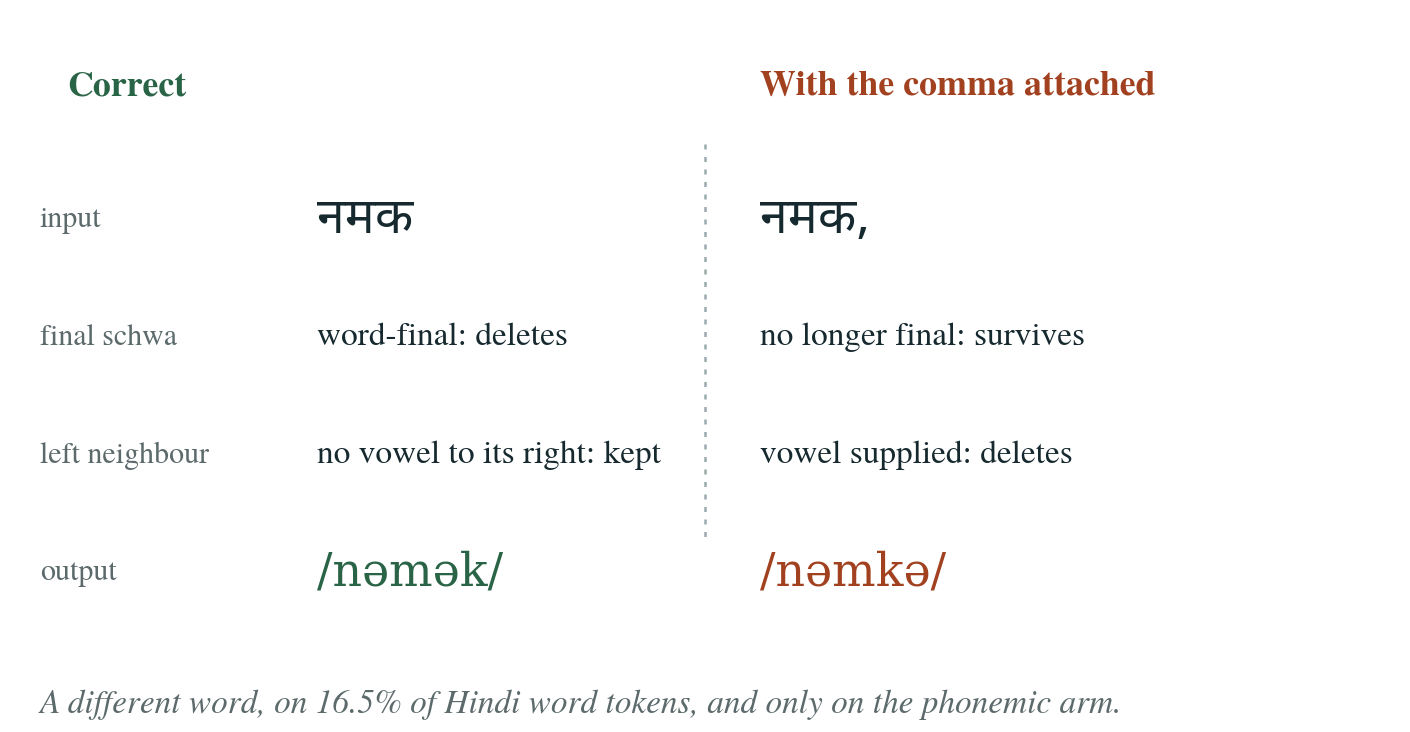
\includegraphics[width=3.85in]{figures/fig_4_2_punctuation_defect.png}
  \caption*{\textbf{Figure 4.1:}  The punctuation defect. With a comma attached, \dev{नमक} came out as \ipa{/nəmkə/} instead of \ipa{/nəmək/}, which is a different word.}
  \addcontentsline{lof}{figure}{Figure 4.1: The punctuation defect}
\end{figure}

The scale is what makes this serious. 16.5 per cent of Hindi word tokens and 14.9 per cent of Marathi carry punctuation, and the damage would have fallen on the phonemic arm alone, because the grapheme path never touches the schwa stage. The headline comparison of this entire study would therefore have been partly measuring the bug, and it would have been measuring it in the direction that made the front end look worse than it is. Punctuation is now stripped from the word edges before the schwa stage and restored afterwards, and there is a parametrised invariance test across nine words and four marks in both languages.

\subsubsection*{5.1.2  A Training Run Was in the Plan Twice}
\addcontentsline{toc}{subsubsection}{5.1.2  A Training Run Was in the Plan Twice}
The design originally had nineteen runs. The nine-hour rung of the ladder was a second copy of the main run under a different identifier: the same architecture, the same data, the same budget, and ten GPU-hours spent on a number that was already in hand. It stayed invisible because the run identifier sat inside the configuration hash, which by construction makes two otherwise identical runs look distinct. The identifier is now excluded from the hash and an assertion refuses any two runs that share a settings hash. The plan came down to seventeen runs and 136 GPU-hours.

\subsubsection*{5.1.3  The Elicitation Sheet Gave Away Its Own Answers}
\addcontentsline{toc}{subsubsection}{5.1.3  The Elicitation Sheet Gave Away Its Own Answers}
The three worked examples at the top of the elicitation sheet were themselves items from the 49-word test set. Every participant would therefore have been handed the correct answers to three of the words they were about to be tested on, and nothing in the merge step would have flagged it. The examples now come from outside the set, and a check at sheet-generation time refuses to write a sheet whose examples appear anywhere in it.

An earlier version of the instrument failed differently. Shown \dev{नमकीन} as \texttt{n[1]m[2]kiin[3]}, the first reader took the numbered blanks to be asking whether a vowel exists anywhere in that syllable, and nearly marked slot 3 yes because of the written ī and slot 1 no even though the word is pronounced with an audible a. Both errors are silent, and with two or three speakers reading it the same way the gold set would have been confidently wrong. The sheet now writes the candidate vowel in place, as \texttt{n(a1)m(a2)kiin(a3)}, which asks a concrete question about a specific sound. An instrument needs piloting on a real reader, not only unit tests.

\subsubsection*{5.1.4  Two Unicode Traps}
\addcontentsline{toc}{subsubsection}{5.1.4  Two Unicode Traps}
Two encoding issues deserve recording because both produce a working program with silently wrong data. Every matra and the virama are Unicode combining marks in categories Mn and Mc [13], for which Python's standard alphanumeric test returns false, so filtering a transcript on that test deletes every vowel sign in the corpus and leaves a bare consonant skeleton without raising anything. The normaliser filters on the Unicode general category instead, and there is a named regression test for it.

The second trap is that the precomposed nukta consonants in the range U+0958 to U+095F are Unicode composition exclusions, which means normalisation form C will not produce them. A literal pasted into source code is therefore already decomposed, so a table keyed on those literals matches nothing and the entire nukta handling becomes a silent no-op. The inventory pins explicit code points rather than literals.

\subsection*{5.2  The Sampling-Rate Confound}
\addcontentsline{toc}{subsection}{5.2  The Sampling-Rate Confound}
This is the one confound in the design that could not be removed, only managed. VITS initialises from a 16 kHz MMS checkpoint, so its output carries nothing above 8 kHz, while FastSpeech 2 and Matcha-TTS run at 22.05 kHz. Three mitigations apply throughout.

\begin{itemize}[leftmargin=1.6em,itemsep=2pt,topsep=3pt]
  \item MCD is reported in two columns, full band and band-limited to 8 kHz, and the band-limited column is the headline comparison. The full-band column is kept so that a reader can see the size of the bandwidth effect rather than having to trust that it was handled.
  \item Listening test stimuli are low-pass filtered to 8 kHz for every system, including the ground-truth anchor, so that raters hear all systems at equal bandwidth.
  \item Word error rate needs no mitigation at all, because Whisper resamples its input to 16 kHz regardless [15].
\end{itemize}

Training VITS from scratch at 22.05 kHz would have removed the confound and introduced a worse one, because VITS would then be the only architecture without a pretrained initialisation and the lower ladder rungs would become a comparison between a pretrained model and an untrained one. Managing the bandwidth difference openly is the smaller cost.

\subsection*{5.3  Threats to Validity}
\addcontentsline{toc}{subsection}{5.3  Threats to Validity}
Seven limitations are worth stating plainly, in roughly descending order of how much they constrain the conclusions.

\begin{enumerate}[leftmargin=1.9em,itemsep=2pt,topsep=3pt]
  \item \textbf{One seed per configuration.} No difference smaller than the measured seed variance will be reported as a finding. With one seed everywhere, that floor has to be established by replicating a single cell and generalising, which is weaker than replicating throughout.
  \item \textbf{The gold set is not yet validated.} Until native speakers have marked the 49 items, the front end's accuracy on contested cases is unknown.
  \item \textbf{VITS is not vocoder-matched.} FastSpeech 2 and Matcha-TTS share one HiFi-GAN; VITS generates its own waveform. The asymmetry is inherent to the architecture.
  \item \textbf{Internal alignment at small data sizes.} As noted in Section 4.7.1, the lowest ladder rungs may suffer more than the top ones from the removal of forced alignment.
  \item \textbf{Single speaker, read speech.} Nothing here generalises to conversational speech or to speaker variation, and no such claim is made.
  \item \textbf{Rare phones in Marathi.} Three phones occur fewer than three times in the corpus and their embedding rows will receive almost no gradient.
  \item \textbf{Predicted MOS is not MOS.} UTMOS and NISQA were trained largely on English and Japanese, so their correlation with human ratings here is itself an open question.
\end{enumerate}

\section*{CHAPTER 6  CONCLUSION AND FUTURE WORK}
\addcontentsline{toc}{section}{Chapter 6  Conclusion and Future Work}
\subsection*{6.1  Conclusion}
\addcontentsline{toc}{subsection}{6.1  Conclusion}
The preparatory phase of this project is complete. Two Devanagari corpora totalling 48.6 hours have been profiled, standardised and split into frozen checksummed partitions that regenerate identically, after recovering a speaker identity that neither dataset records. The front end is built with schwa deletion isolated as a switchable stage and covers both corpora with zero unknown symbols across 870,547 phone tokens. Both objective metrics have been verified against analytic answers rather than merely executed. All seventeen runs are specified and the shared budget is enforced by assertion.

Three defects turned up along the way and none of them announced itself. The worst affected 16.5 per cent of Hindi word tokens and would have degraded only the phonemic arm, which is precisely the half of the comparison this study rests on. All three were found the same way, by running the code over the real corpus or by watching somebody try to use an instrument, and the 78 unit tests caught none of them. Each now has a regression test or an assertion behind it.

Nothing has been trained. That is deliberate ordering rather than delay: every property in Chapter 4 had to be established before GPU time was spent, because a defect in the corpus, the front end or a metric would have propagated silently into everything that followed. The apparatus has already earned that caution three times over.

\subsection*{6.2  Immediate Work}
\addcontentsline{toc}{subsection}{6.2  Immediate Work}
\begin{enumerate}[leftmargin=1.9em,itemsep=2pt,topsep=3pt]
  \item Write the four training wrappers, for FastSpeech 2, VITS, Matcha-TTS and HiFi-GAN, each reading one run configuration and writing resumable checkpoints. None of this needs a GPU.
  \item Complete the evaluation harness: word error rate against its ground-truth floor, predicted mean opinion score, and real-time factor.
  \item Write the analysis code and the statistical treatment before any numbers arrive, so that the analysis is not chosen after seeing the results.
  \item Build the listening test infrastructure and pilot it on two or three people before recruiting a full panel.
  \item Collect elicitation sheets from two or three native Hindi speakers, which turns the 49-item set from self-consistent into validated. This is blocked on people, not on code.
  \item Verify the GPU execution path end to end, including the checkpoint round trip described in Section 3.9.
\end{enumerate}

\subsection*{6.3  Future Work}
\addcontentsline{toc}{subsection}{6.3  Future Work}
Four extensions are worth naming, in the order they would be worth doing.

\begin{itemize}[leftmargin=1.6em,itemsep=2pt,topsep=3pt]
  \item \textbf{Three seeds throughout.} At 368 GPU-hours this is out of reach on free-tier resources and inside a few days on an institutional accelerator. It converts the variance floor from an assumption into a measurement, and it is the first thing extra compute should buy.
  \item \textbf{StyleTTS 2.} Excluded here for compute, as set out in Section 2.1.4. Adding it would test whether the front-end effect survives into the strongest current architecture.
  \item \textbf{Sanskrit.} The original synopsis paired Hindi with Classical Sanskrit, which was moved to future work because its data sits behind a request process with unknown turnaround. Marathi is the better control in any case, because it differs from Hindi in the rule rather than in the resource level.
  \item \textbf{Other implicit orthographic processes.} Schwa deletion is one of several places where Devanagari underspecifies pronunciation. The pattern used here, holding everything fixed and moving only the input representation while adding a same-script control, transfers to any of them.
\end{itemize}

Whichever way the main result goes, it is useful. If the architectures absorb schwa deletion from data, nobody building an Indic TTS system needs to write that front end again, and this report will say so with a measurement behind it. If they do not, the field should stop defaulting to character level input for Indic languages.

\section*{REFERENCES}
\addcontentsline{toc}{section}{References}
\begin{singlespace}
\begin{enumerate}[label={[\arabic*]},leftmargin=2.3em,itemsep=3pt,topsep=4pt]
  \item B. Narasimhan, R. Sproat and G. Kiraz, “Schwa-deletion in Hindi text-to-speech synthesis,” \textit{International Journal of Speech Technology}, vol. 7, no. 4, pp. 319–333, 2004.
  \item A. Arora, L. Gessler and N. Schneider, “Supervised grapheme-to-phoneme conversion of orthographic schwas in Hindi and Punjabi,” in \textit{Proc. Annual Meeting of the Association for Computational Linguistics (ACL)}, 2020, pp. 7791–7795, arXiv:2004.10353.
  \item Y. Ren, C. Hu, X. Tan et al., “FastSpeech 2: Fast and high-quality end-to-end text to speech,” in \textit{Proc. International Conference on Learning Representations (ICLR)}, 2021, arXiv:2006.04558.
  \item J. Kim, J. Kong and J. Son, “Conditional variational autoencoder with adversarial learning for end-to-end text-to-speech,” in \textit{Proc. International Conference on Machine Learning (ICML)}, 2021, pp. 5530–5540, arXiv:2106.06103.
  \item S. Mehta, R. Tu, J. Beskow et al., “Matcha-TTS: A fast TTS architecture with conditional flow matching,” in \textit{Proc. IEEE International Conference on Acoustics, Speech and Signal Processing (ICASSP)}, 2024, pp. 11341–11345, arXiv:2309.03199.
  \item J. Kong, J. Kim and J. Bae, “HiFi-GAN: Generative adversarial networks for efficient and high fidelity speech synthesis,” in \textit{Advances in Neural Information Processing Systems (NeurIPS)}, vol. 33, 2020, pp. 17022–17033, arXiv:2010.05646.
  \item A. Baby, A. L. Thomas, N. L. Nishanthi et al., “Resources for Indian languages,” in \textit{Proc. Text, Speech and Dialogue (CBBLR Workshop)}, 2016, pp. 37–43.
  \item G. K. Kumar, P. S. V., P. Kumar et al., “Towards building text-to-speech systems for the next billion users,” in \textit{Proc. IEEE International Conference on Acoustics, Speech and Signal Processing (ICASSP)}, 2023, arXiv:2211.09536.
  \item A. Sankar, S. Anand, P. Varadhan et al., “IndicVoices-R: Unlocking a massive multilingual multi-speaker speech corpus for scaling Indian TTS,” in \textit{Advances in Neural Information Processing Systems (NeurIPS), Datasets and Benchmarks Track}, 2024, arXiv:2409.05356.
  \item V. Pratap, A. Tjandra, B. Shi et al., “Scaling speech technology to 1,000+ languages,” \textit{Journal of Machine Learning Research}, vol. 25, no. 97, pp. 1–52, 2024, arXiv:2305.13516.
  \item M. Ohala, “Hindi,” in \textit{Handbook of the International Phonetic Association}, Cambridge, U.K.: Cambridge University Press, 1999, pp. 100–103.
  \item R. V. Dhongde and K. Wali, \textit{Marathi} (London Oriental and African Language Library, vol. 13). Amsterdam, The Netherlands: John Benjamins, 2009.
  \item The Unicode Consortium, \textit{The Unicode Standard, Version 15.1.0}, Chapter 12: South and Central Asia–I. Mountain View, CA, USA: Unicode Consortium, 2023.
  \item R. Kubichek, “Mel-cepstral distance measure for objective speech quality assessment,” in \textit{Proc. IEEE Pacific Rim Conference on Communications, Computers and Signal Processing}, vol. 1, 1993, pp. 125–128.
  \item A. Radford, J. W. Kim, T. Xu et al., “Robust speech recognition via large-scale weak supervision,” in \textit{Proc. International Conference on Machine Learning (ICML)}, 2023, pp. 28492–28518, arXiv:2212.04356.
  \item M. McAuliffe, M. Socolof, S. Mihuc et al., “Montreal Forced Aligner: Trainable text-speech alignment using Kaldi,” in \textit{Proc. Interspeech}, 2017, pp. 498–502.
  \item J. Shen, R. Pang, R. J. Weiss et al., “Natural TTS synthesis by conditioning WaveNet on mel spectrogram predictions,” in \textit{Proc. IEEE International Conference on Acoustics, Speech and Signal Processing (ICASSP)}, 2018, pp. 4779–4783, arXiv:1712.05884.
  \item J. Kim, S. Kim, J. Kong and S. Yoon, “Glow-TTS: A generative flow for text-to-speech via monotonic alignment search,” in \textit{Advances in Neural Information Processing Systems (NeurIPS)}, vol. 33, 2020, pp. 8067–8077, arXiv:2005.11129.
  \item Y. Lipman, R. T. Q. Chen, H. Ben-Hamu et al., “Flow matching for generative modeling,” in \textit{Proc. International Conference on Learning Representations (ICLR)}, 2023, arXiv:2210.02747.
  \item Y. A. Li, C. Han, V. S. Raghavan et al., “StyleTTS 2: Towards human-level text-to-speech through style diffusion and adversarial training with large speech language models,” in \textit{Advances in Neural Information Processing Systems (NeurIPS)}, vol. 36, 2023, arXiv:2306.07691.
  \item R. Badlani, A. Łańcucki, K. J. Shih et al., “One TTS alignment to rule them all,” in \textit{Proc. IEEE International Conference on Acoustics, Speech and Signal Processing (ICASSP)}, 2022, pp. 6092–6096, arXiv:2108.10447.
  \item H. Sakoe and S. Chiba, “Dynamic programming algorithm optimization for spoken word recognition,” \textit{IEEE Transactions on Acoustics, Speech and Signal Processing}, vol. 26, no. 1, pp. 43–49, 1978.
  \item J. Kominek, T. Schultz and A. W. Black, “Synthesizer voice quality of new languages calibrated with mean mel cepstral distortion,” in \textit{Proc. Workshop on Spoken Languages Technologies for Under-Resourced Languages (SLTU)}, 2008, pp. 63–68.
  \item M. Morise, F. Yokomori and K. Ozawa, “WORLD: A vocoder-based high-quality speech synthesis system for real-time applications,” \textit{IEICE Transactions on Information and Systems}, vol. E99-D, no. 7, pp. 1877–1884, 2016.
  \item M. Mauch and S. Dixon, “pYIN: A fundamental frequency estimator using probabilistic threshold distributions,” in \textit{Proc. IEEE International Conference on Acoustics, Speech and Signal Processing (ICASSP)}, 2014, pp. 659–663.
  \item T. Saeki, D. Xin, W. Nakata et al., “UTMOS: UTokyo-SaruLab system for VoiceMOS Challenge 2022,” in \textit{Proc. Interspeech}, 2022, pp. 4521–4525, arXiv:2204.02152.
  \item G. Mittag, B. Naderi, A. Chehadi and S. Möller, “NISQA: A deep CNN-self-attention model for multidimensional speech quality prediction with crowdsourced datasets,” in \textit{Proc. Interspeech}, 2021, pp. 2127–2131, arXiv:2104.09494.
  \item International Telecommunication Union, “Methods for subjective determination of transmission quality,” Recommendation ITU-T P.800, Geneva, Switzerland, 1996.
  \item International Telecommunication Union, “Algorithms to measure audio programme loudness and true-peak audio level,” Recommendation ITU-R BS.1770-4, Geneva, Switzerland, 2015.
  \item European Broadcasting Union, “Loudness normalisation and permitted maximum level of audio signals,” EBU Recommendation R 128, Geneva, Switzerland, 2020.
\end{enumerate}
\end{singlespace}
\clearpage
\section*{APPENDIX A  RUN CONFIGURATION MATRIX}
\addcontentsline{toc}{section}{Appendix A  Run Configuration Matrix}
Every run is defined by one YAML file. The fields below are shared by all acoustic runs and are compared by an assertion at generation time; a mismatch in any of them refuses to write the configuration files.

\begin{Verbatim}[fontsize=\small,xleftmargin=1.5em]
budget:
  max_steps:        100000
  batch_frames:     12000
  lr:               2.0e-4
  lr_schedule:      warmup_inverse_sqrt
  warmup_steps:     4000
  precision:        fp16
  grad_clip:        1.0

cosmetic_fields_excluded_from_hash:
  - notes
  - created
  - run_id          # excluded so that duplicate runs are detectable
\end{Verbatim}

Table A.1 lists the seventeen runs with the fields that differ between them.

\begin{table}[htbp]
  \centering
  \footnotesize
  \caption*{\textbf{Table A.1:}  Per-run settings.}
  \addcontentsline{lot}{table}{Table A.1: Per-run settings}
  \begin{tabular}{p{0.58in}p{1.33in}p{0.58in}p{1.13in}p{0.73in}p{0.63in}}
  \toprule
  \textbf{Run} & \textbf{Arch.} & \textbf{Lang.} & \textbf{Input} & \textbf{Rung} & \textbf{Rate} \\
  \midrule
  r01 & FastSpeech 2 & hi & phonemic & 9 h & 22.05 \\
  r02 & VITS & hi & phonemic & 9 h & 16 \\
  r03 & Matcha-TTS & hi & phonemic & 9 h & 22.05 \\
  r04 & FastSpeech 2 & hi & graphemic & 9 h & 22.05 \\
  r05 & VITS & hi & graphemic & 9 h & 16 \\
  r06 & HiFi-GAN & hi & GT mel & 9 h & 22.05 \\
  r07 & FastSpeech 2 & hi & phonemic & 5 h & 22.05 \\
  r08 & FastSpeech 2 & hi & phonemic & 1 h & 22.05 \\
  r09 & FastSpeech 2 & hi & phonemic & 30 min & 22.05 \\
  r10 & FastSpeech 2 & hi & phonemic & 10 min & 22.05 \\
  r11 & VITS & hi & phonemic & 5 h & 16 \\
  r12 & VITS & hi & phonemic & 1 h & 16 \\
  r13 & VITS & hi & phonemic & 30 min & 16 \\
  r14 & VITS & hi & phonemic & 10 min & 16 \\
  r15 & FastSpeech 2 & mr & phonemic & 9 h & 22.05 \\
  r16 & VITS & mr & phonemic & 9 h & 16 \\
  r17 & HiFi-GAN & mr & GT mel & 9 h & 22.05 \\
  \bottomrule
  \end{tabular}
\end{table}

\section*{APPENDIX B  PHONE INVENTORY}
\addcontentsline{toc}{section}{Appendix B  Phone Inventory}
The inventory declares 75 symbols. Hindi uses 72 of them and Marathi 67, and Marathi's set is a strict subset of Hindi's. The five symbols Marathi does not use are marked below.

\begin{table}[htbp]
  \centering
  \small
  \caption*{\textbf{Table B.1:}  Declared phone inventory, grouped by class.}
  \addcontentsline{lot}{table}{Table B.1: Declared phone inventory, grouped by class}
  \begin{tabular}{p{1.63in}p{4.00in}}
  \toprule
  \textbf{Class} & \textbf{Symbols} \\
  \midrule
  Plosives, unaspirated & p  b  \ipa{t̪}  \ipa{d̪}  \ipa{ʈ}  \ipa{ɖ}  k  \ipa{ɡ} \\
  Plosives, aspirated & \ipa{pʰ}  \ipa{bʱ}  \ipa{t̪ʰ}  \ipa{d̪ʱ}  \ipa{ʈʰ}  \ipa{ɖʱ}  \ipa{kʰ}  \ipa{ɡʱ} \\
  Affricates & \ipa{tʃ}  \ipa{dʒ}  \ipa{tʃʰ}  \ipa{dʒʱ} \\
  Nasals & m  n  \ipa{ɳ}  \ipa{ɲ}  ŋ \\
  Fricatives & f  s  z*  \ipa{ʃ}  \ipa{ʂ}  \ipa{ɦ}  x*  \ipa{ɣ}* \\
  Approximants and laterals & \ipa{ʋ}  j  l  \ipa{ɭ}  r  \ipa{ɾ}  \ipa{ɾʱ}  \ipa{ɽ}*  \ipa{ɽʱ}* \\
  Vowels, short & \ipa{ə}  \ipa{ɪ}  \ipa{ʊ}  e  o \\
  Vowels, long & \ipa{aː}  \ipa{iː}  \ipa{uː}  \ipa{eː}  \ipa{oː}  \ipa{ɛː}  \ipa{ɔː} \\
  Nasalised vowels & \ipa{ə̃}  \ipa{aː̃}  \ipa{iː̃}  \ipa{uː̃}  \ipa{eː̃}  \ipa{oː̃}  \ipa{ɛː̃}  \ipa{ɔː̃} \\
  Prosody and boundary & ,  .  ?  !  word boundary  utterance boundary \\
  \bottomrule
  \end{tabular}
  \par\vspace{3pt}\begin{minipage}{5.95in}\footnotesize\itshape Symbols marked * do not occur in the Marathi corpus. The vocalic \ipa{r̥} and a small number of Perso-Arabic symbols are declared but occur fewer than three times in Marathi, which is recorded as a weakness in Section 4.5.\end{minipage}
\end{table}

\section*{APPENDIX C  ELICITATION SHEET}
\addcontentsline{toc}{section}{Appendix C  Elicitation Sheet}
The sheet below is generated for each speaker. It never shows the rule's prediction. The three worked examples at the top are checked at generation time against the test set and the sheet is refused if any of them appears in it.

\begin{Verbatim}[fontsize=\small,xleftmargin=1.5em]
CONTESTED SCHWA ELICITATION  —  speaker __________   date __________

For each numbered slot, say the word aloud the way you normally would and mark:
    Y  the vowel (a) IS pronounced there
    N  the vowel (a) is NOT pronounced there
    V  it varies / both sound acceptable to me

Vowels that are plainly written are NOT in question. Only the bracketed (a) slots are.

WORKED EXAMPLES (not part of the test)
  kap(a1)r(a2)aa   1: N  2: N      bart(a1)n(a2)   1: N  2: Y      paanii   no slots

ITEMS
   1.  n(a1)m(a2)k(a3)        1: ___  2: ___  3: ___
   2.  n(a1)m(a2)kiin(a3)     1: ___  2: ___  3: ___
   3.  s(a1)m(a2)jh(a3)naa    1: ___  2: ___  3: ___
  ...  (49 items in total)
\end{Verbatim}

Answers are merged through the same converter that produces the phonemic arm's symbols, so the IPA comes from the inventory and only the judgement is human.

\section*{APPENDIX D  SCHWA DELETION PSEUDOCODE}
\addcontentsline{toc}{section}{Appendix D  Schwa Deletion Pseudocode}
The implementation follows the rule of Narasimhan, Sproat and Kiraz [1] with an unconditional word-final deletion applied first and a lexicon override applied last. The \texttt{delete\_medial} flag is False for Marathi and True for Hindi, and is the whole of the control condition.

\begin{Verbatim}[fontsize=\small,xleftmargin=1.5em]
function delete_schwas(segments, config):
    # segments carry .phone, .inherent (True for an unwritten schwa)

    if config.delete_final:
        i = last index where segments[i].inherent
        if i exists and count_vowels(segments) > config.min_vowels:
            mark segments[i] deleted

    if not config.delete_medial:
        return survivors(segments)          # Marathi stops here

    for i from len(segments) - 1 down to 0:  # right to left
        if not segments[i].inherent:  continue
        if segments[i] already deleted: continue
        if segments[i].phone in config.block_before: continue

        left  = nearest live segment before i
        right = nearest live segment after  i
        if left is a consonant preceded by a live vowel
           and right is a consonant followed by a live vowel:
               mark segments[i] deleted

    return survivors(segments)
\end{Verbatim}

The loop runs right to left because a deletion removes the vowel that the next candidate to its left would have needed, which blocks that candidate. Running left to right produces \textit{samjhana} for \dev{समझना} instead of \textit{samajhna}. The invariance test added after the punctuation defect asserts that stripping and restoring punctuation around a word leaves the phone sequence unchanged, across nine words and four marks in both languages.

\end{document}
